\documentclass[12pt, letter]{report}
\usepackage[utf8]{inputenc}
\usepackage[final]{pdfpages}

\begin{document}	
\begin{titlepage}	
	\begin{center}
		\huge UNIVERSIDAD AUTÓNOMA DE NUEVO LEÓN\\
		\bigskip
		\bigskip
		FACULTAD DE INGENIERÍA MECÁNICA Y ELÉCTRICA\\
		\bigskip
		\bigskip
		POSGRADO EN INGENIERÍA DE SISTEMAS ... \\
		\bigskip
		\bigskip
		\bigskip
		\bigskip
		\begin{Large}
			PORTAFOLIO DE EVIDENCIAS DE ANÁLISIS ESTADÍSTICO MULTIVARIADO... \\
		\end{Large}
		\bigskip
		\bigskip
		\begin{large}
		\bigskip
			PROFESOR(A): DRA. SATU ELISA SCHAEFFER\\
		\bigskip
		\end{large}
		\bigskip
		\bigskip
		\bigskip
		\begin{large}
			AUTOR: LUIS ÁNGEL GUTIÉRREZ RODRÍGUEZ\\
			MATRICULA: 1484412\\
		\end{large}
	\end{center}	
\end{titlepage}	





\chapter*{Introducción}

El siguiente documento es el portafolio de evidencias de la materia Análisis Estadístico Multivariado. El curso constó de 14 actividades, 13 proyectos en Jupyter Notebook y la redacción de un articulo de carácter científico en Latex. El cual fue co-evaluado por la Doctora Schaeffer y el grupo del curso.

Este portafolio consiste en anexar las actividades revisadas por la Dra. Schaeffer. Después detallar la experiencia adquirida al realizar la práctica. Finalmente, si es posible, se anexarán las mismas actividades pero corrigiendo los errores antes cometidos y que fueron señalados por la Dra. Schaeffer.


\newpage

\chapter*{Práctica 1: Preparación de datos}

\section*{Complicaciones}
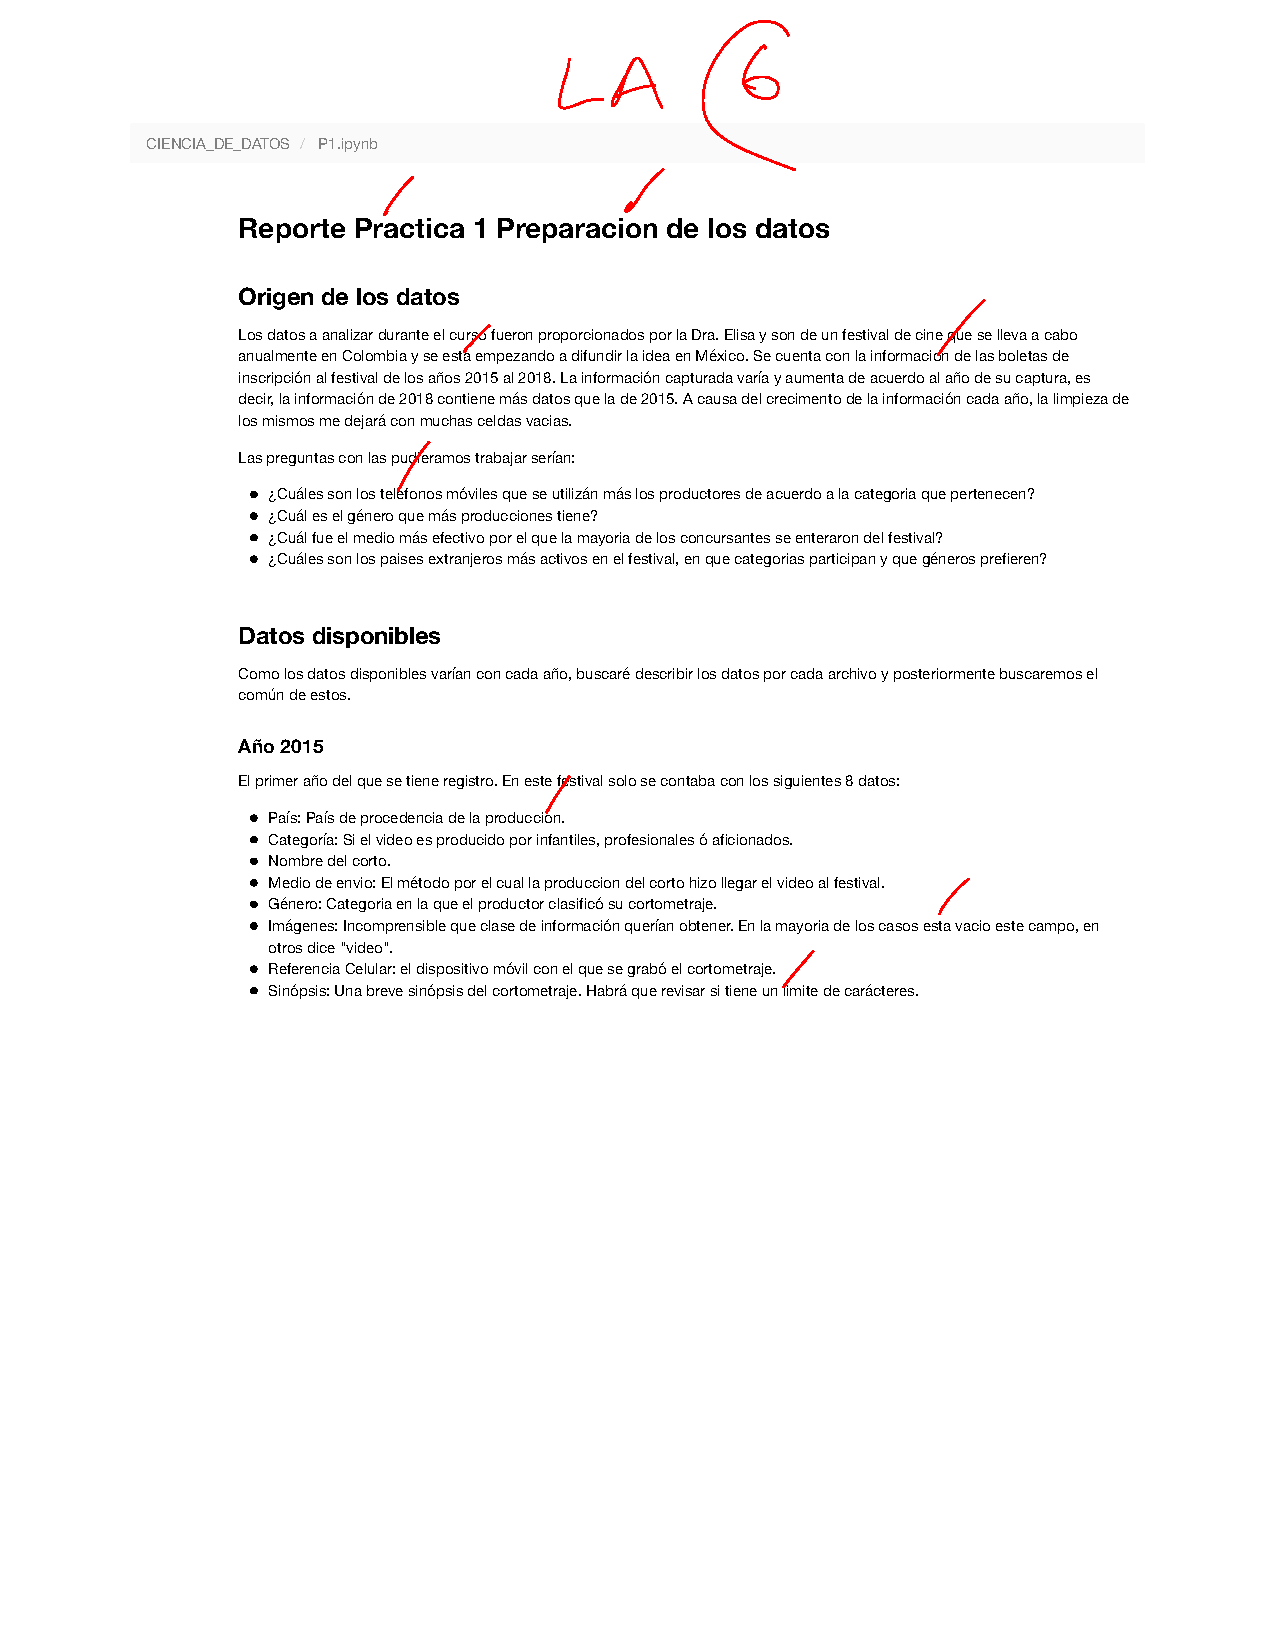
\includepdf[ pages=-, frame, scale=.85]{LA1}
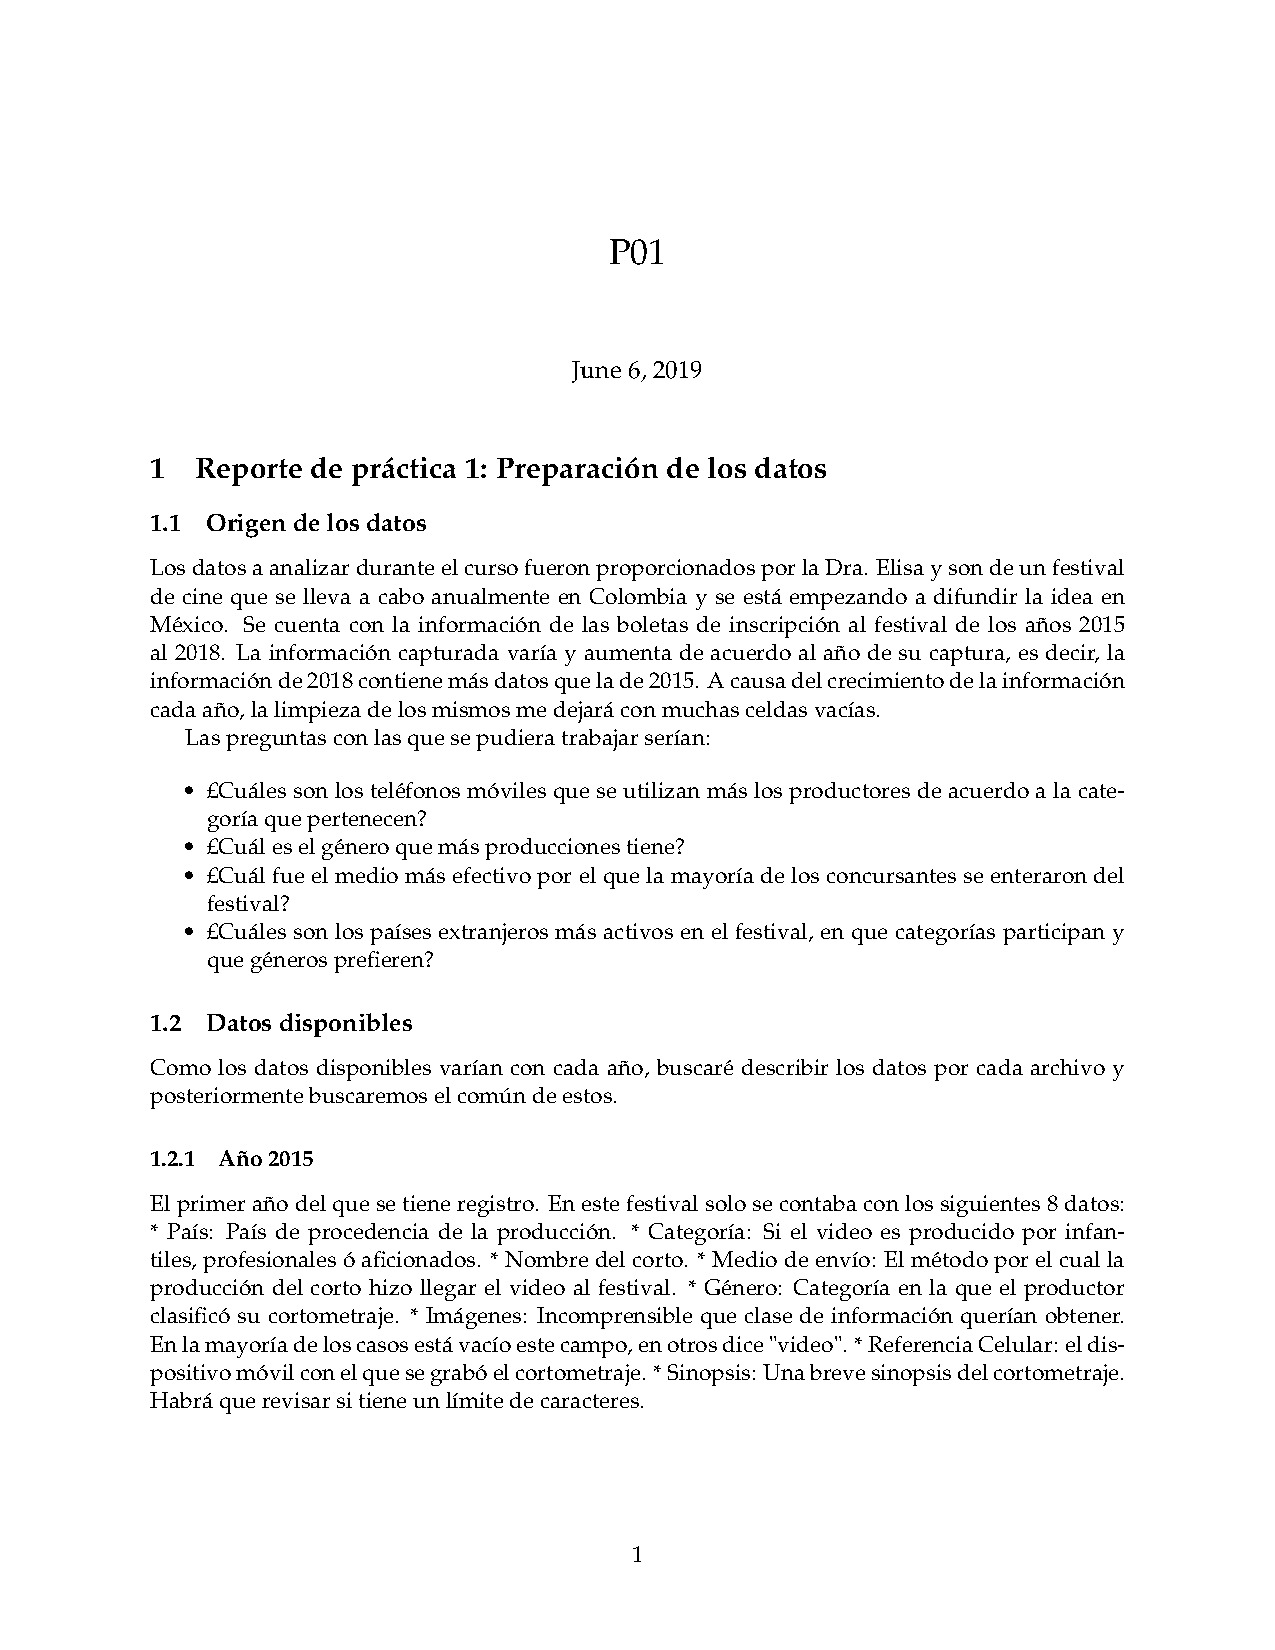
\includepdf[ pages=-, frame, scale=.85]{P01}

\chapter*{Práctica 2: Lectura y manipulación de datos}
\section*{Complicaciones}
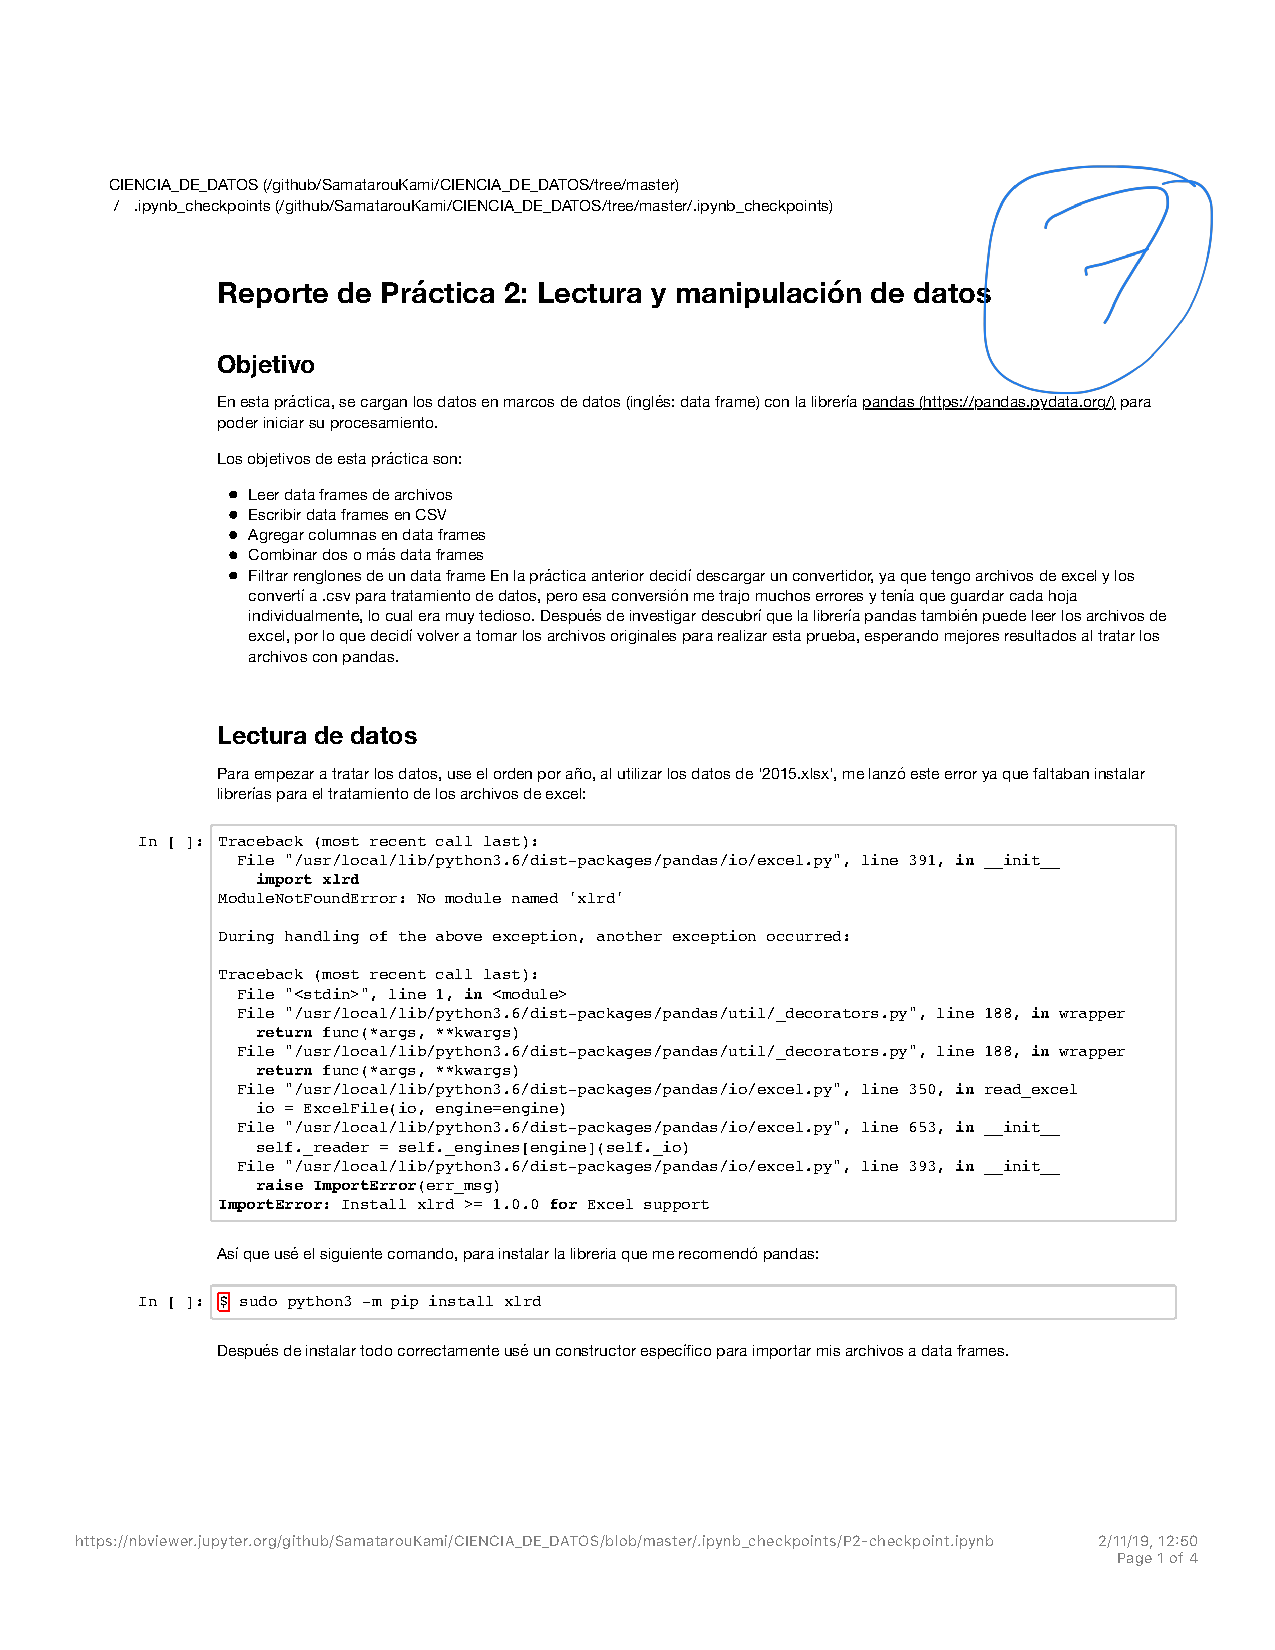
\includepdf[ pages=-, frame, scale=.85]{LA2}
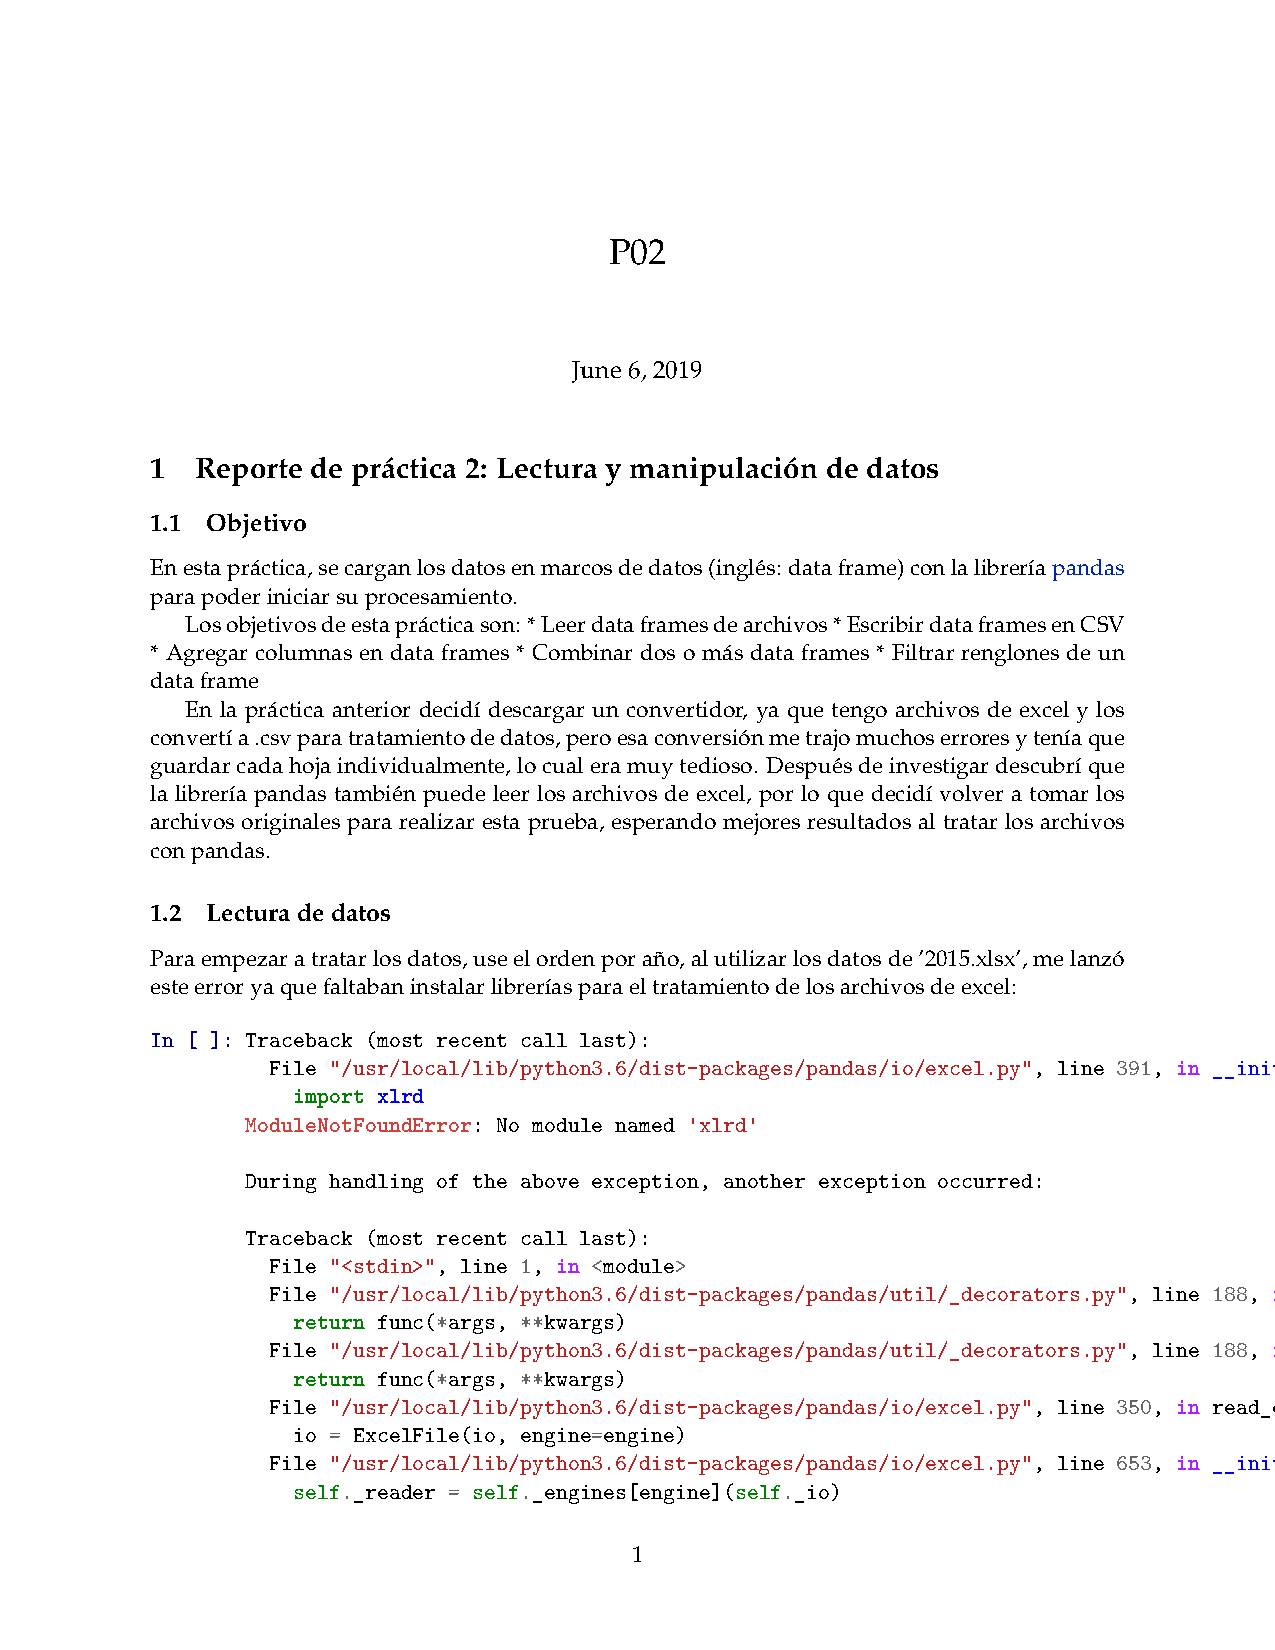
\includepdf[ pages=-, frame, scale=.85]{P02}

\chapter*{Práctica 3: Estadística descriptiva básica}
\section*{Complicaciones}
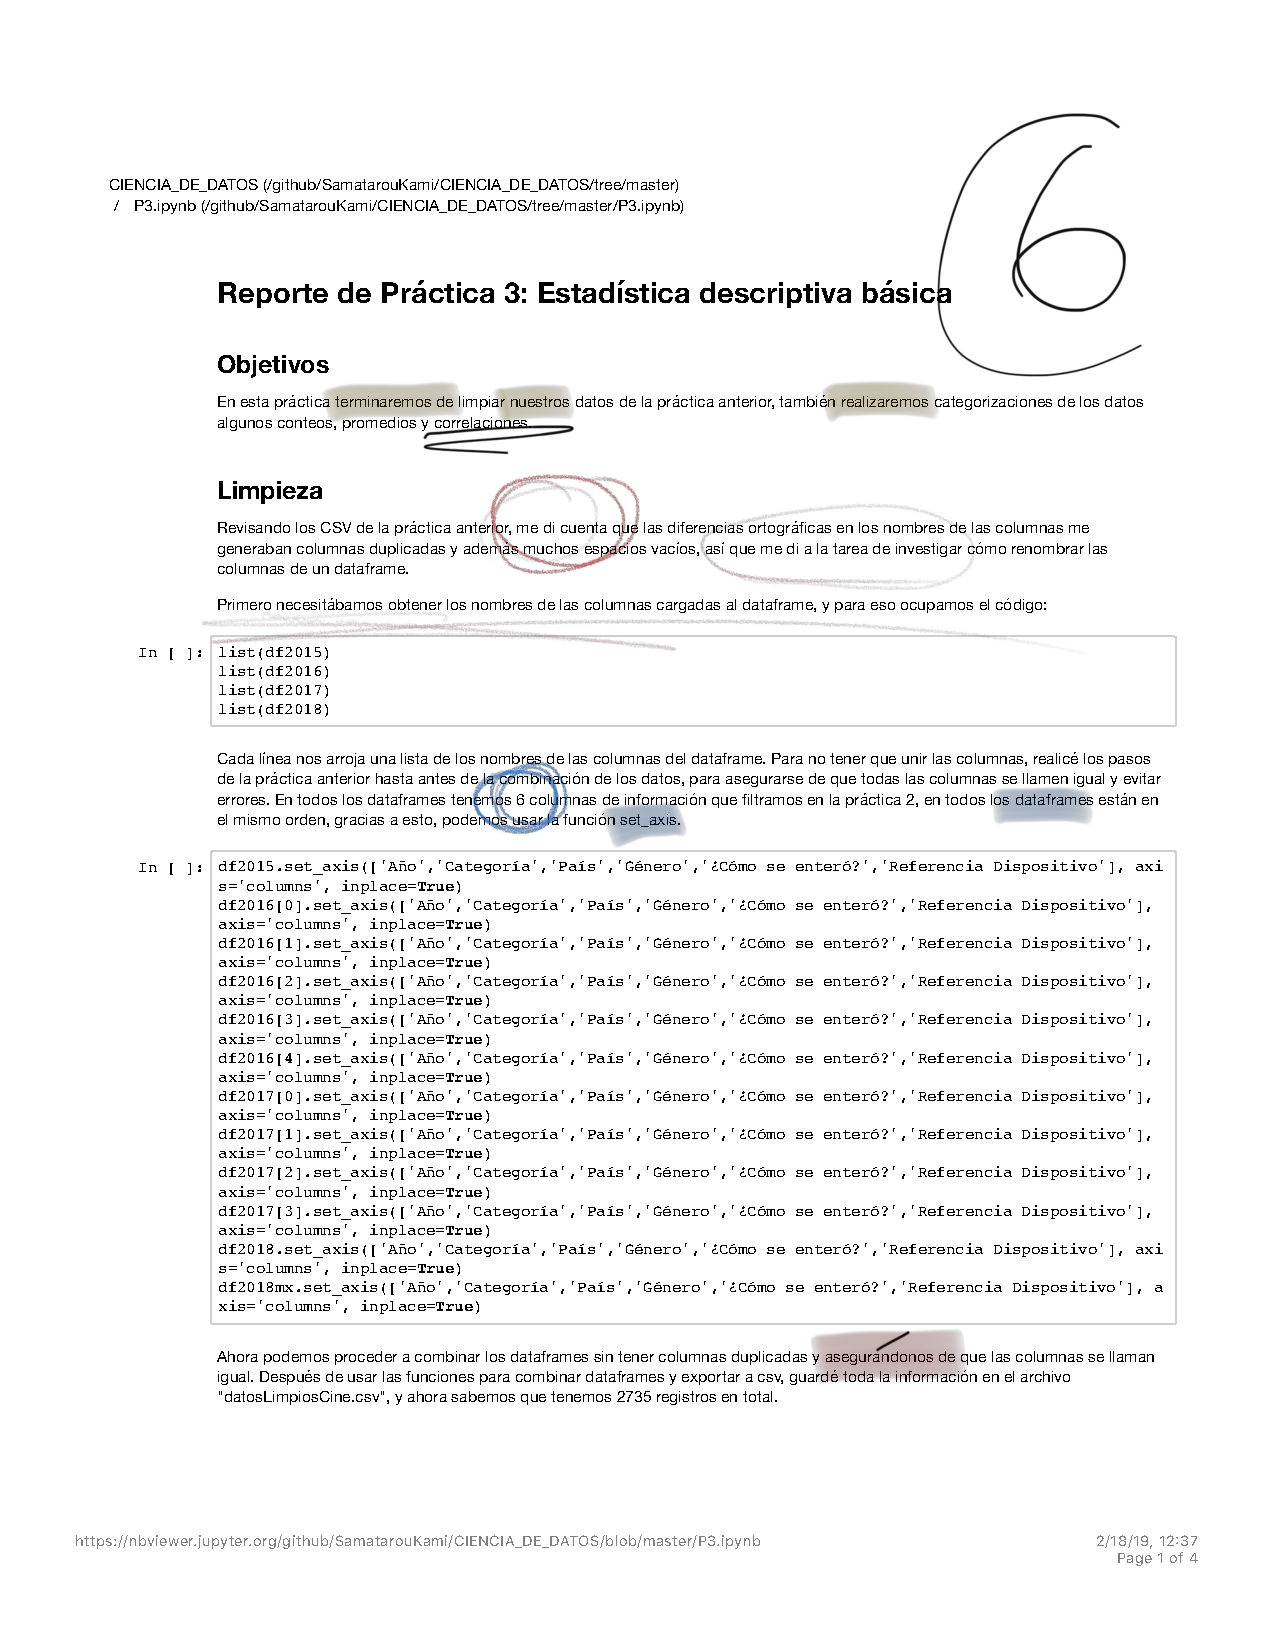
\includepdf[ pages=-, frame, scale=.85]{LA3}
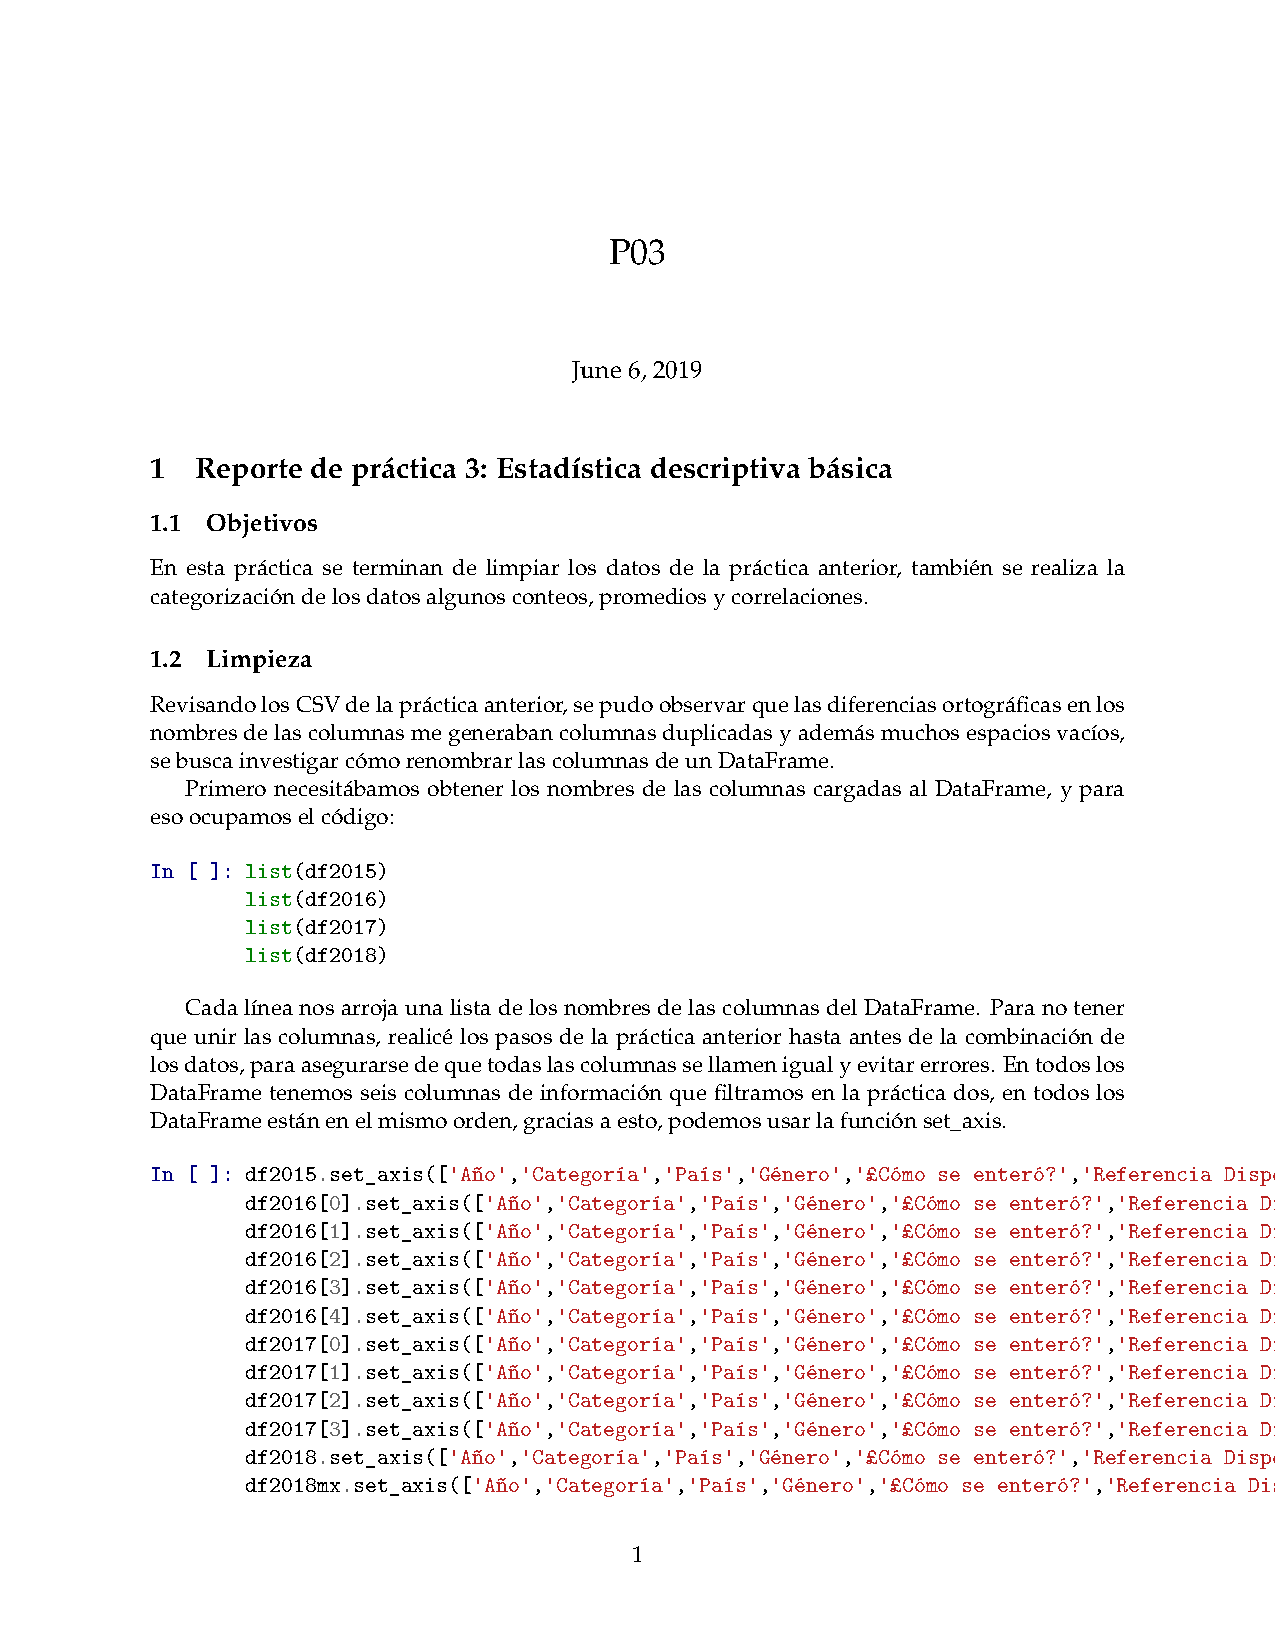
\includepdf[ pages=-, frame, scale=.85]{P03}

\chapter*{Práctica 4: Visualización de información}
\section*{Complicaciones}

\includepdf[ pages=-, frame, scale=.85]{NP}
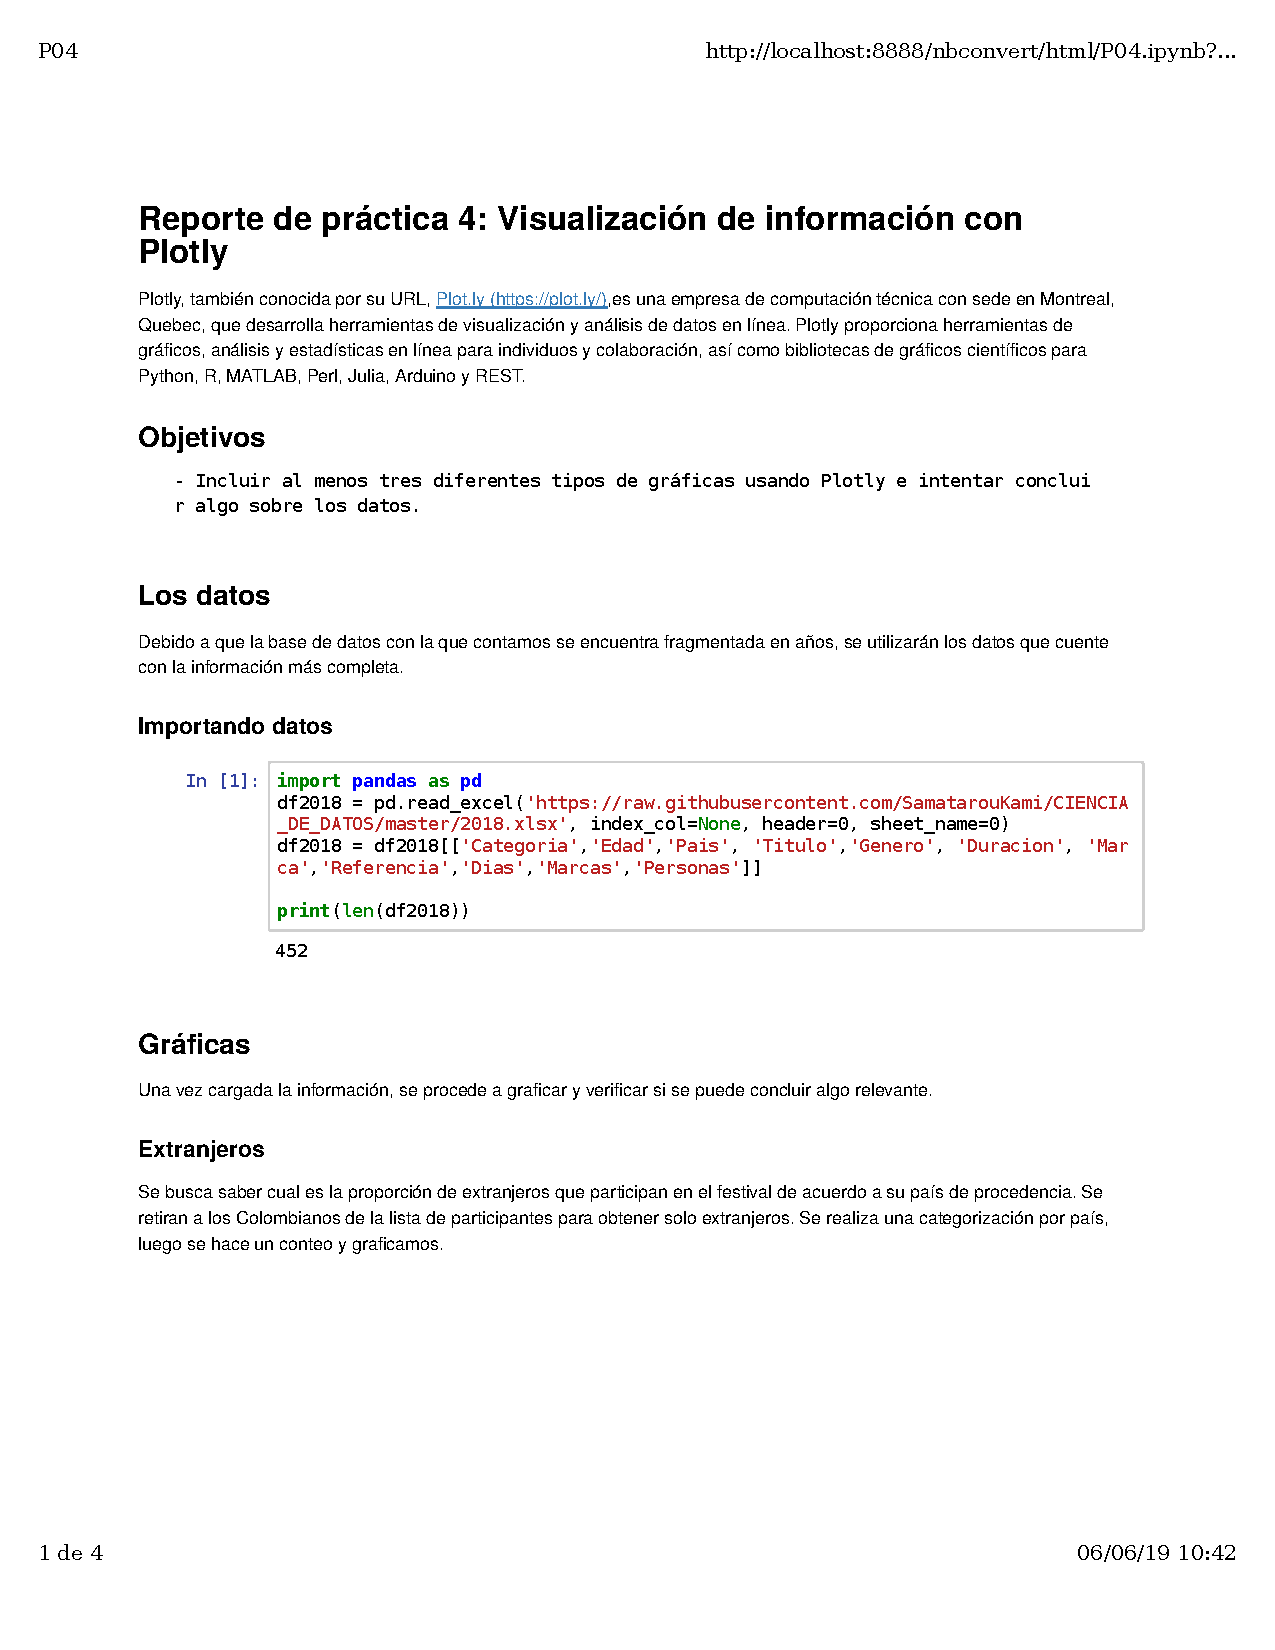
\includepdf[ pages=-, frame, scale=.85]{P04}

\chapter*{Práctica 5: Pruebas estadísticas}
\section*{Complicaciones}
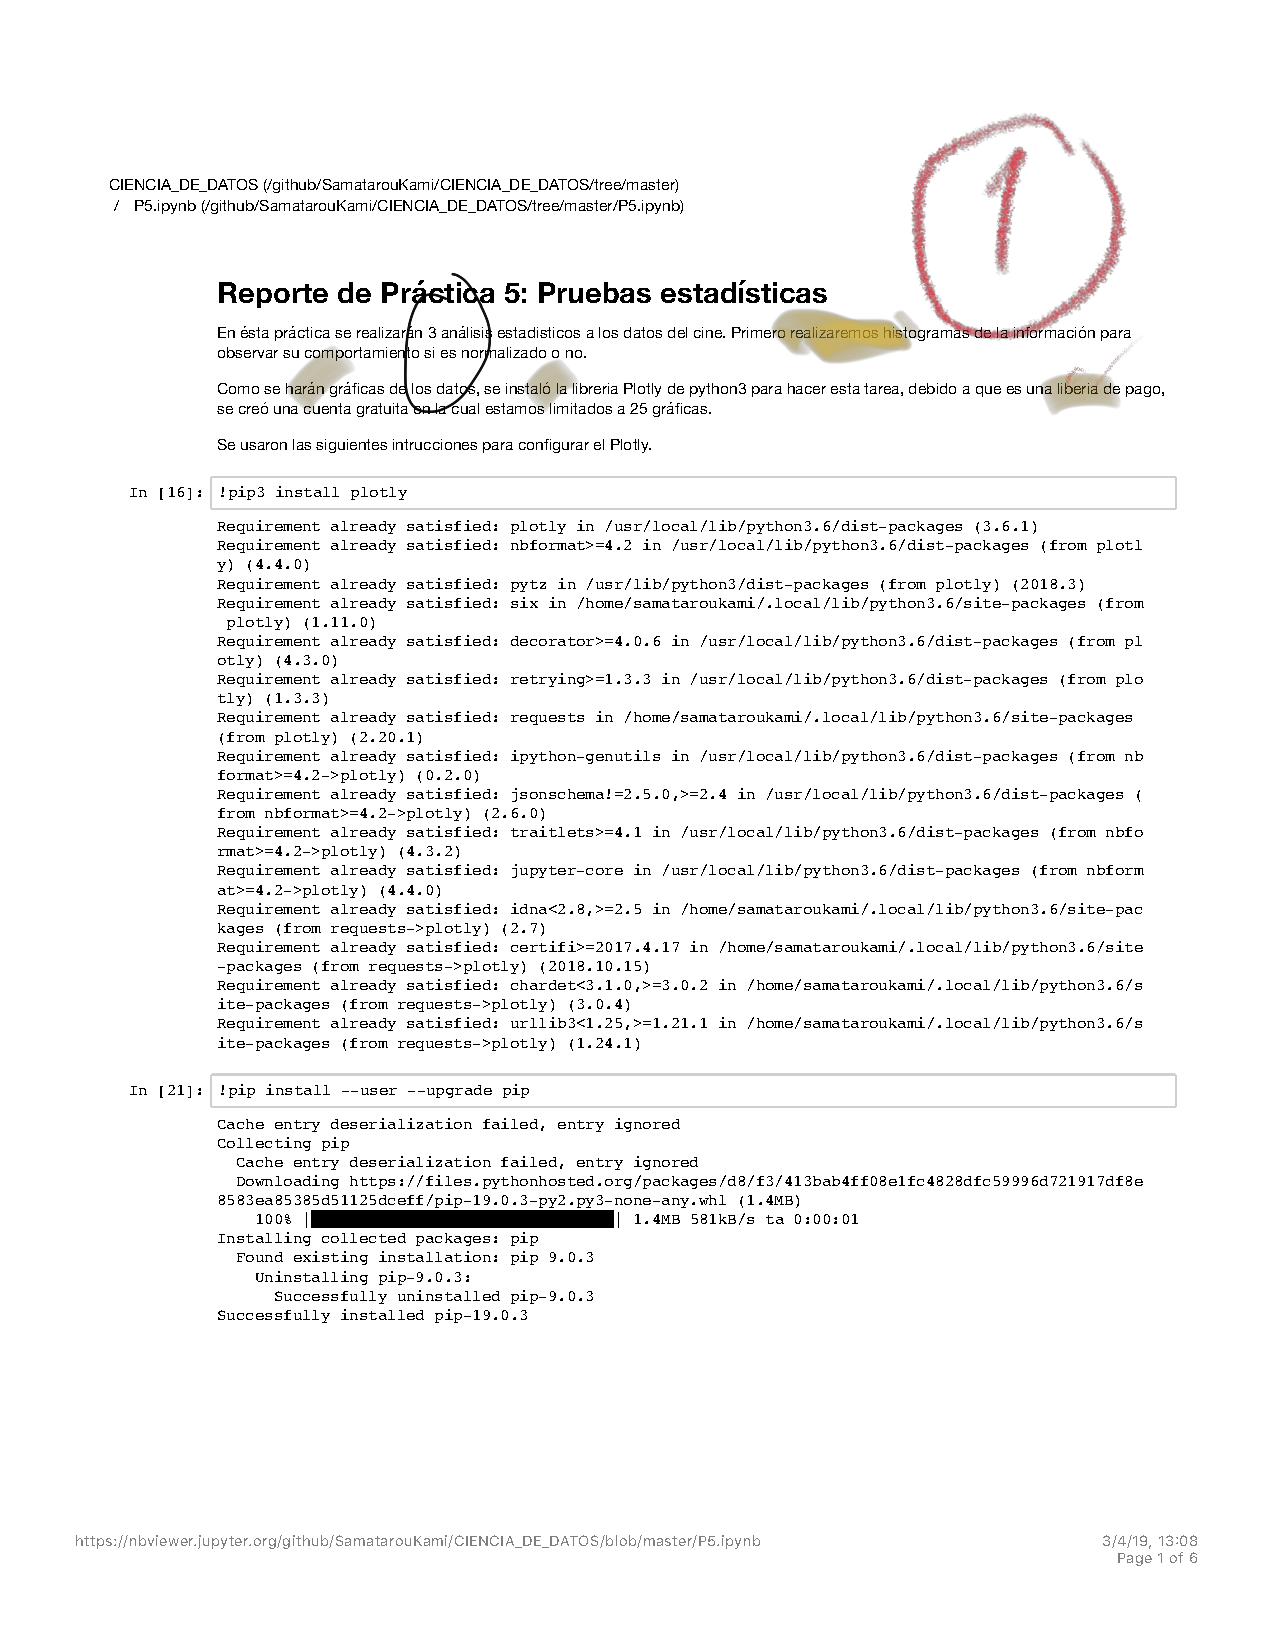
\includepdf[ pages=-, frame, scale=.85]{LA5}
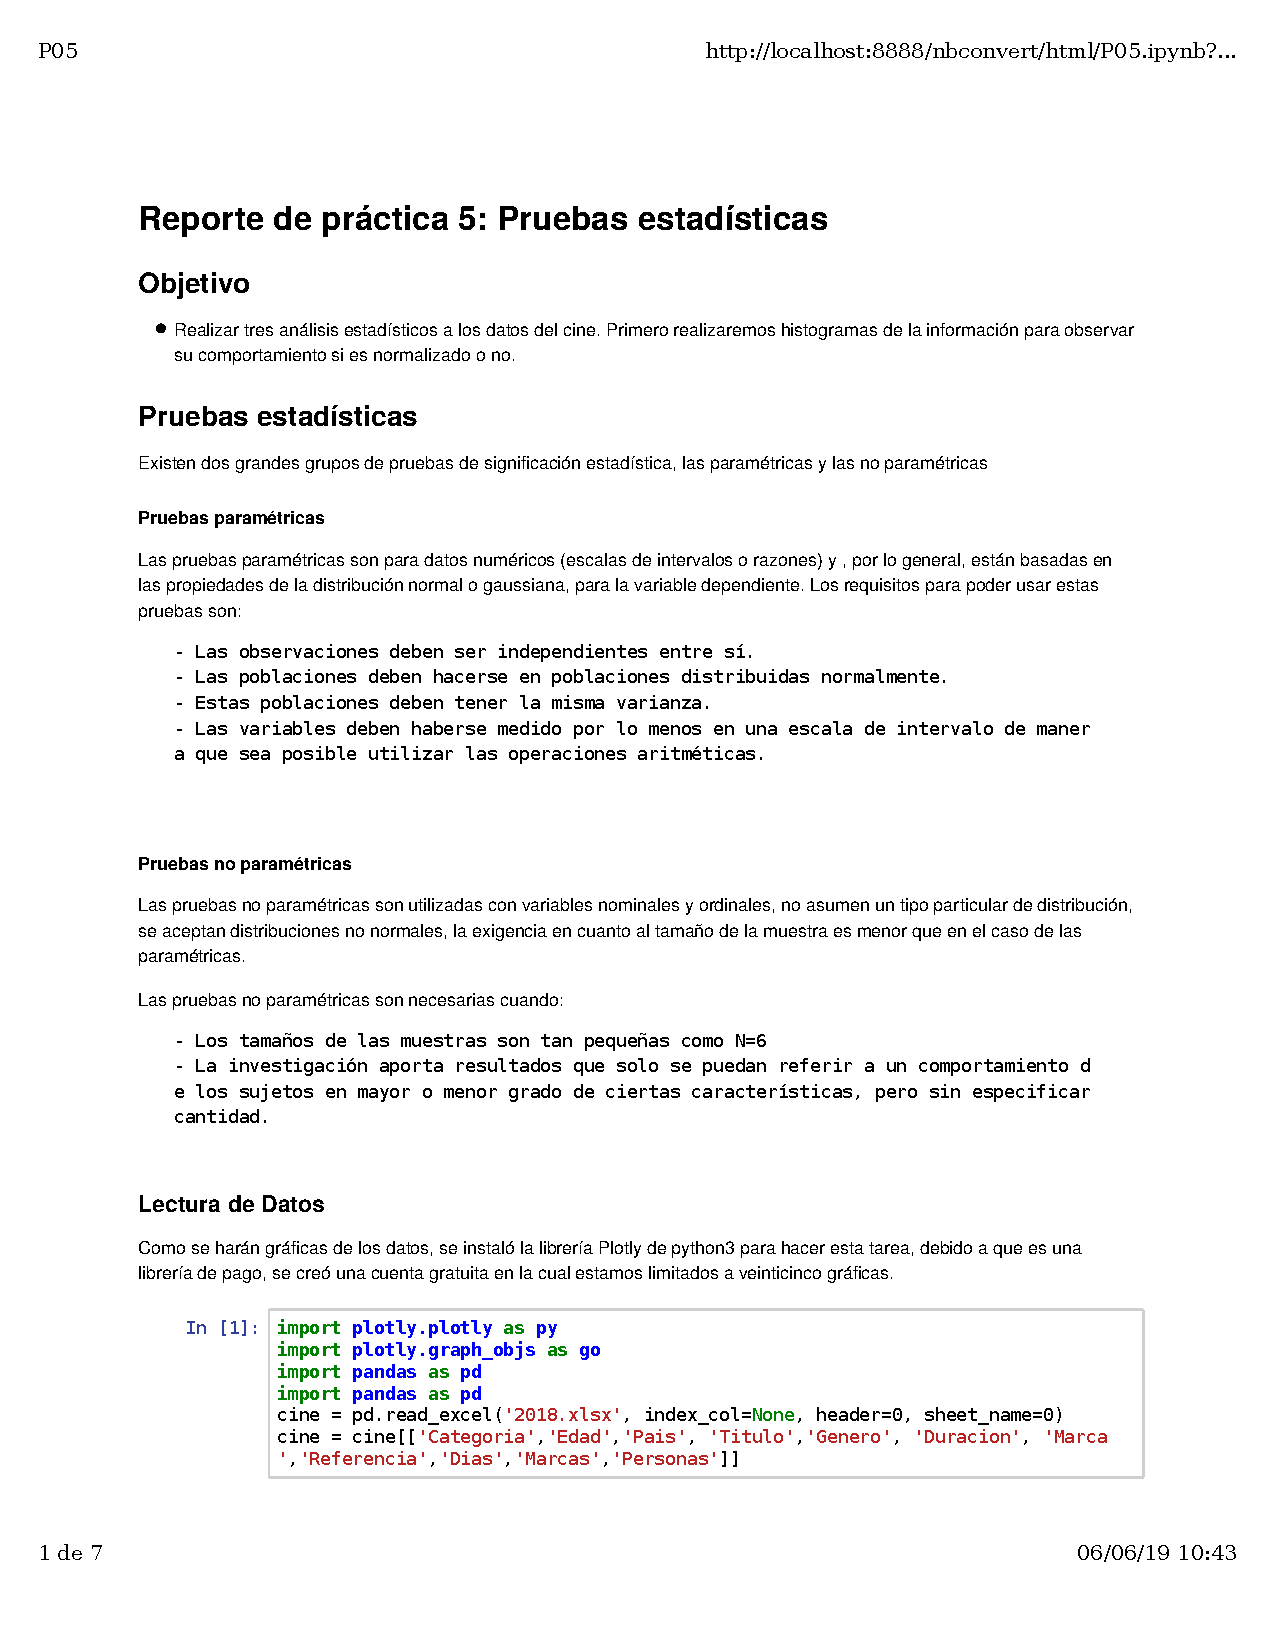
\includepdf[ pages=-, frame, scale=.85]{P05}

\chapter*{Práctica 6: Modelos lineales}
\section*{Complicaciones}
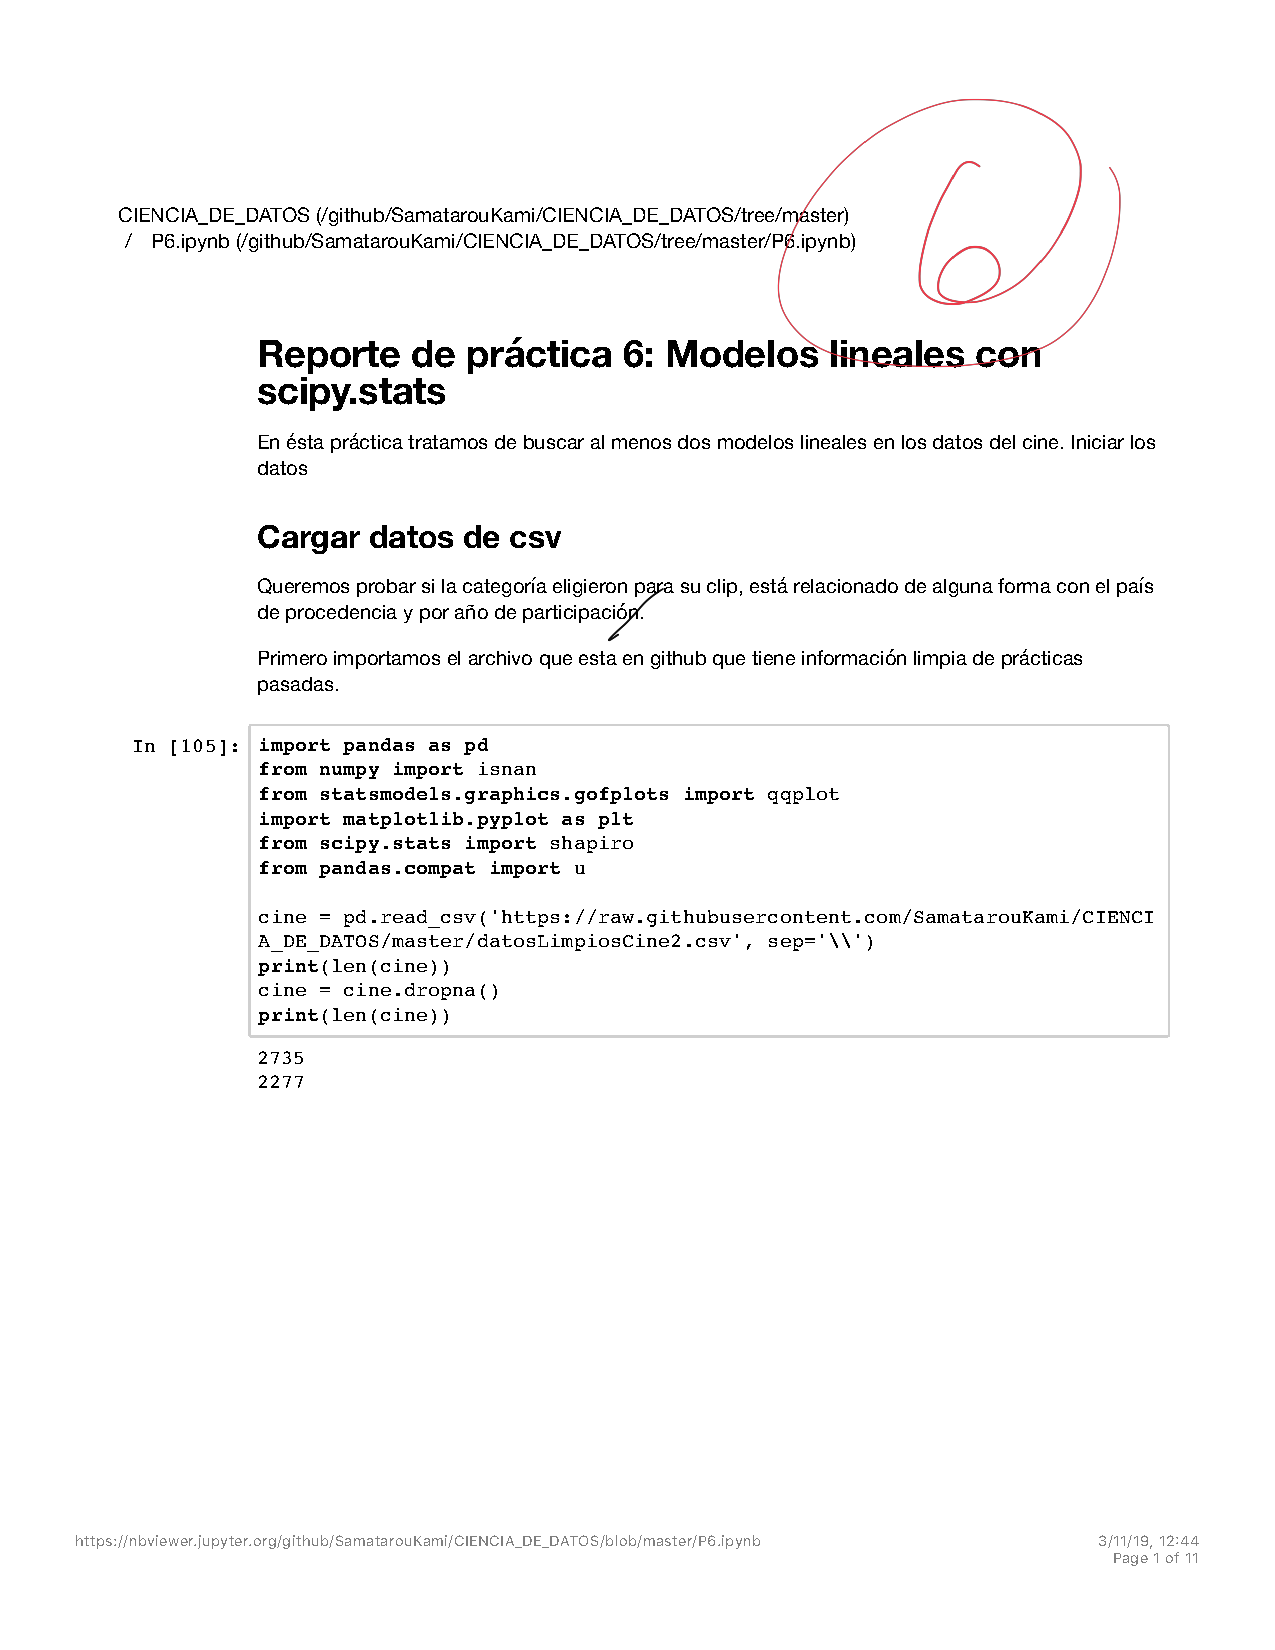
\includepdf[ pages=-, frame, scale=.85]{LA6}
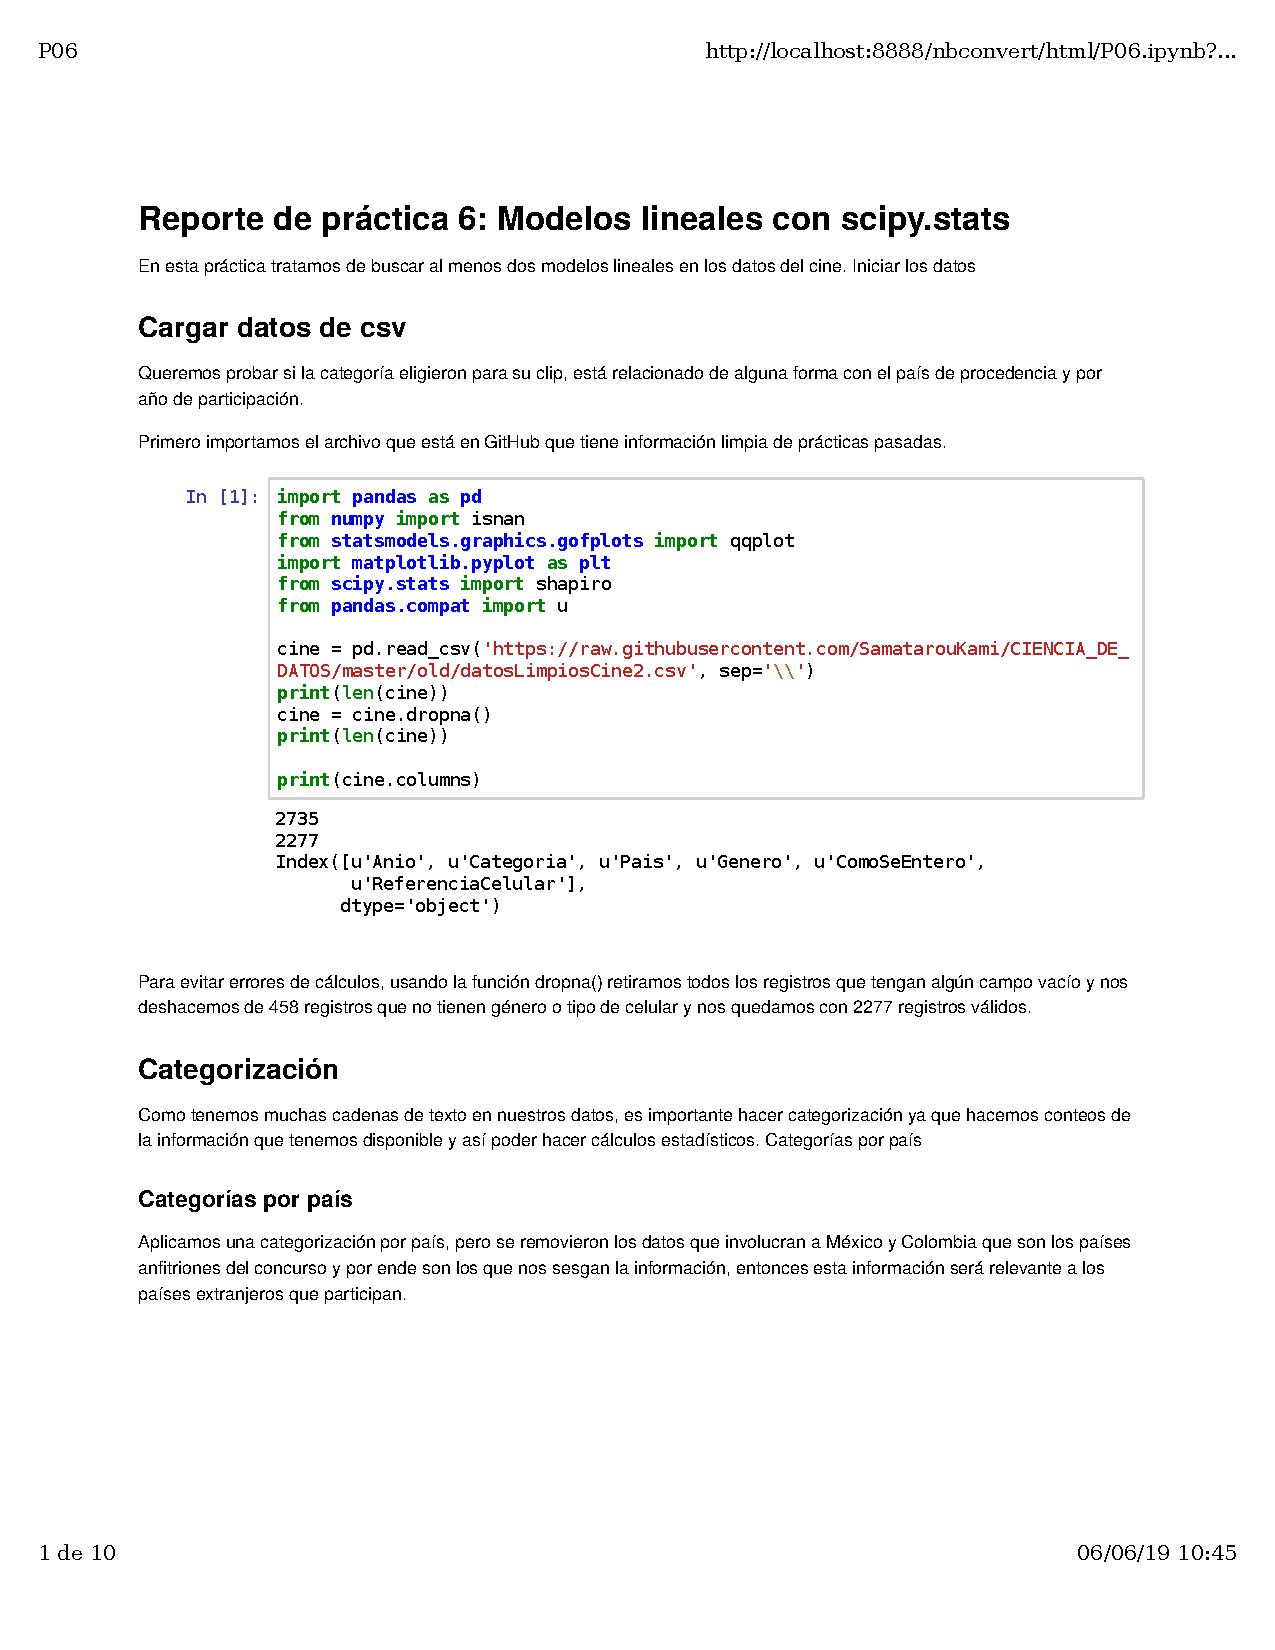
\includepdf[ pages=-, frame, scale=.85]{P06}

\chapter*{Práctica 7: Regresión múltiple}
\section*{Complicaciones}
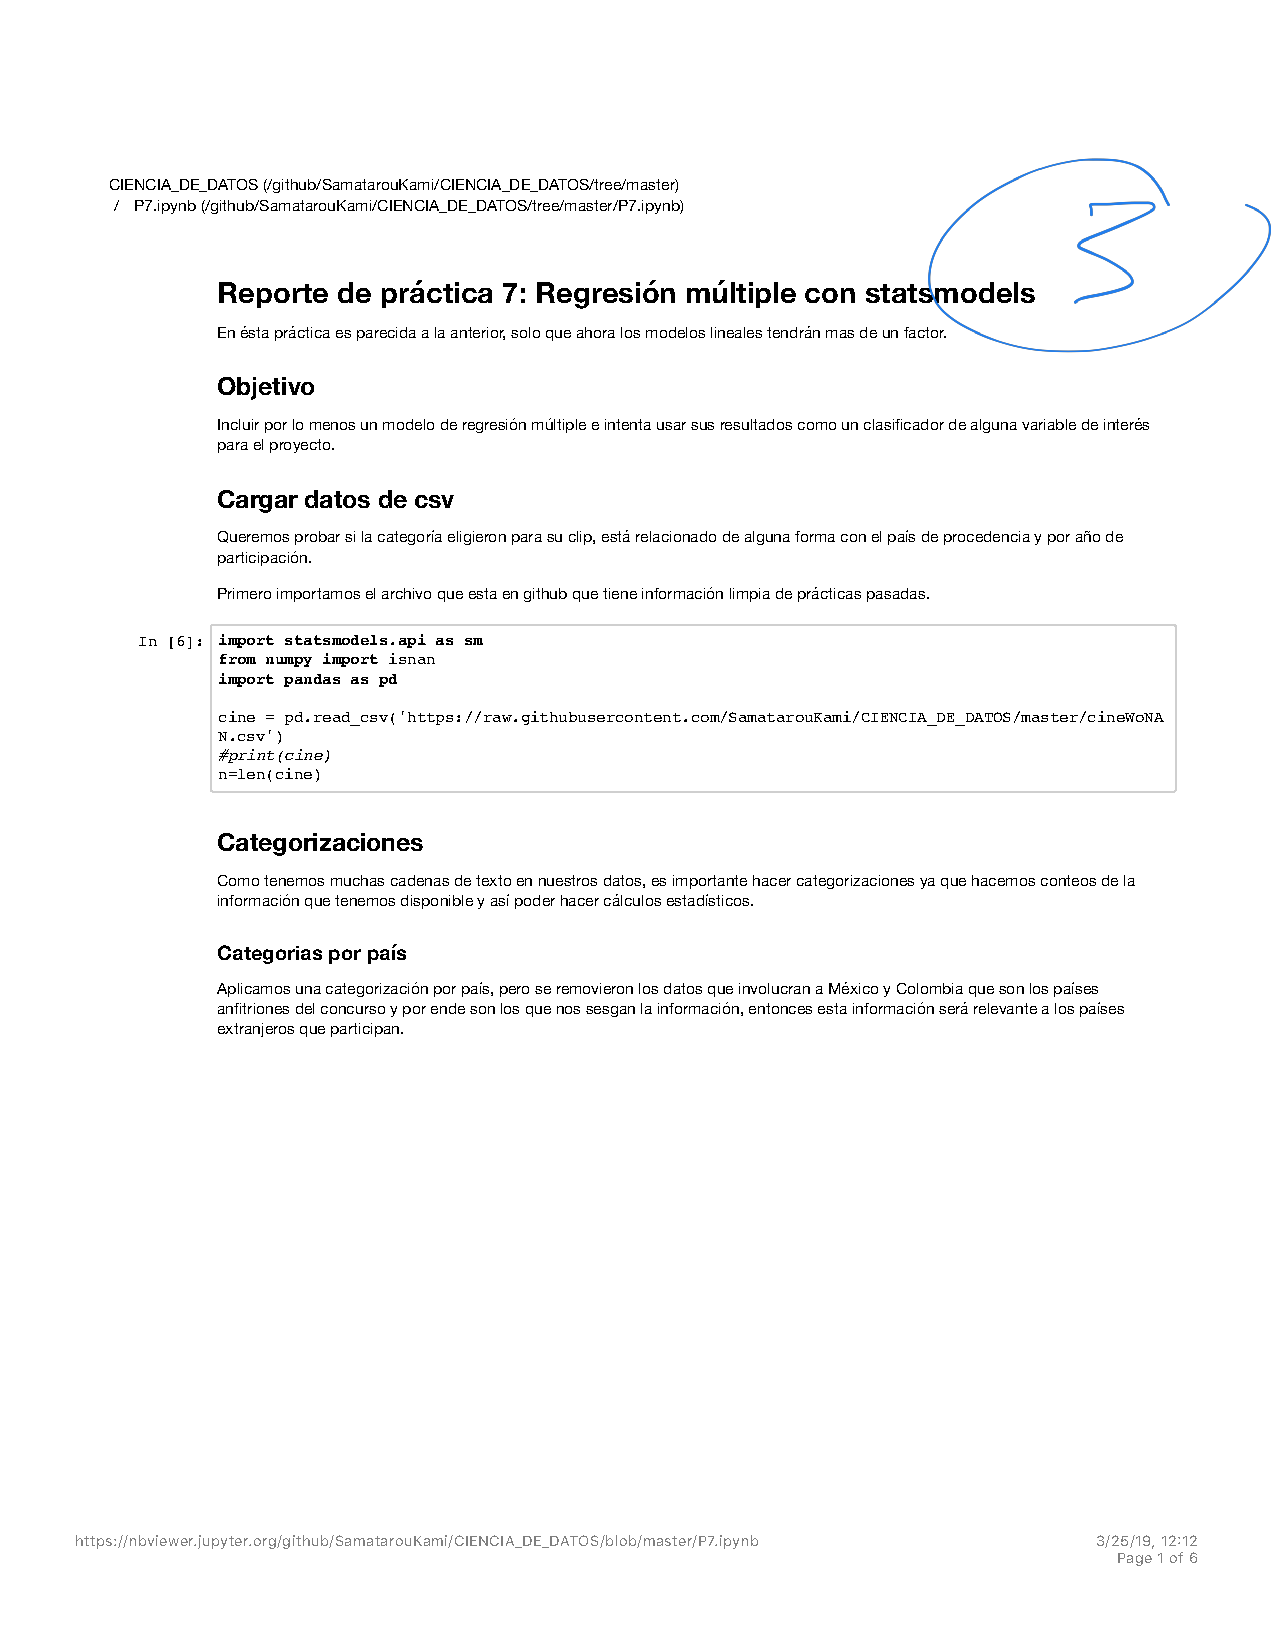
\includepdf[ pages=-, frame, scale=.85]{LA7}
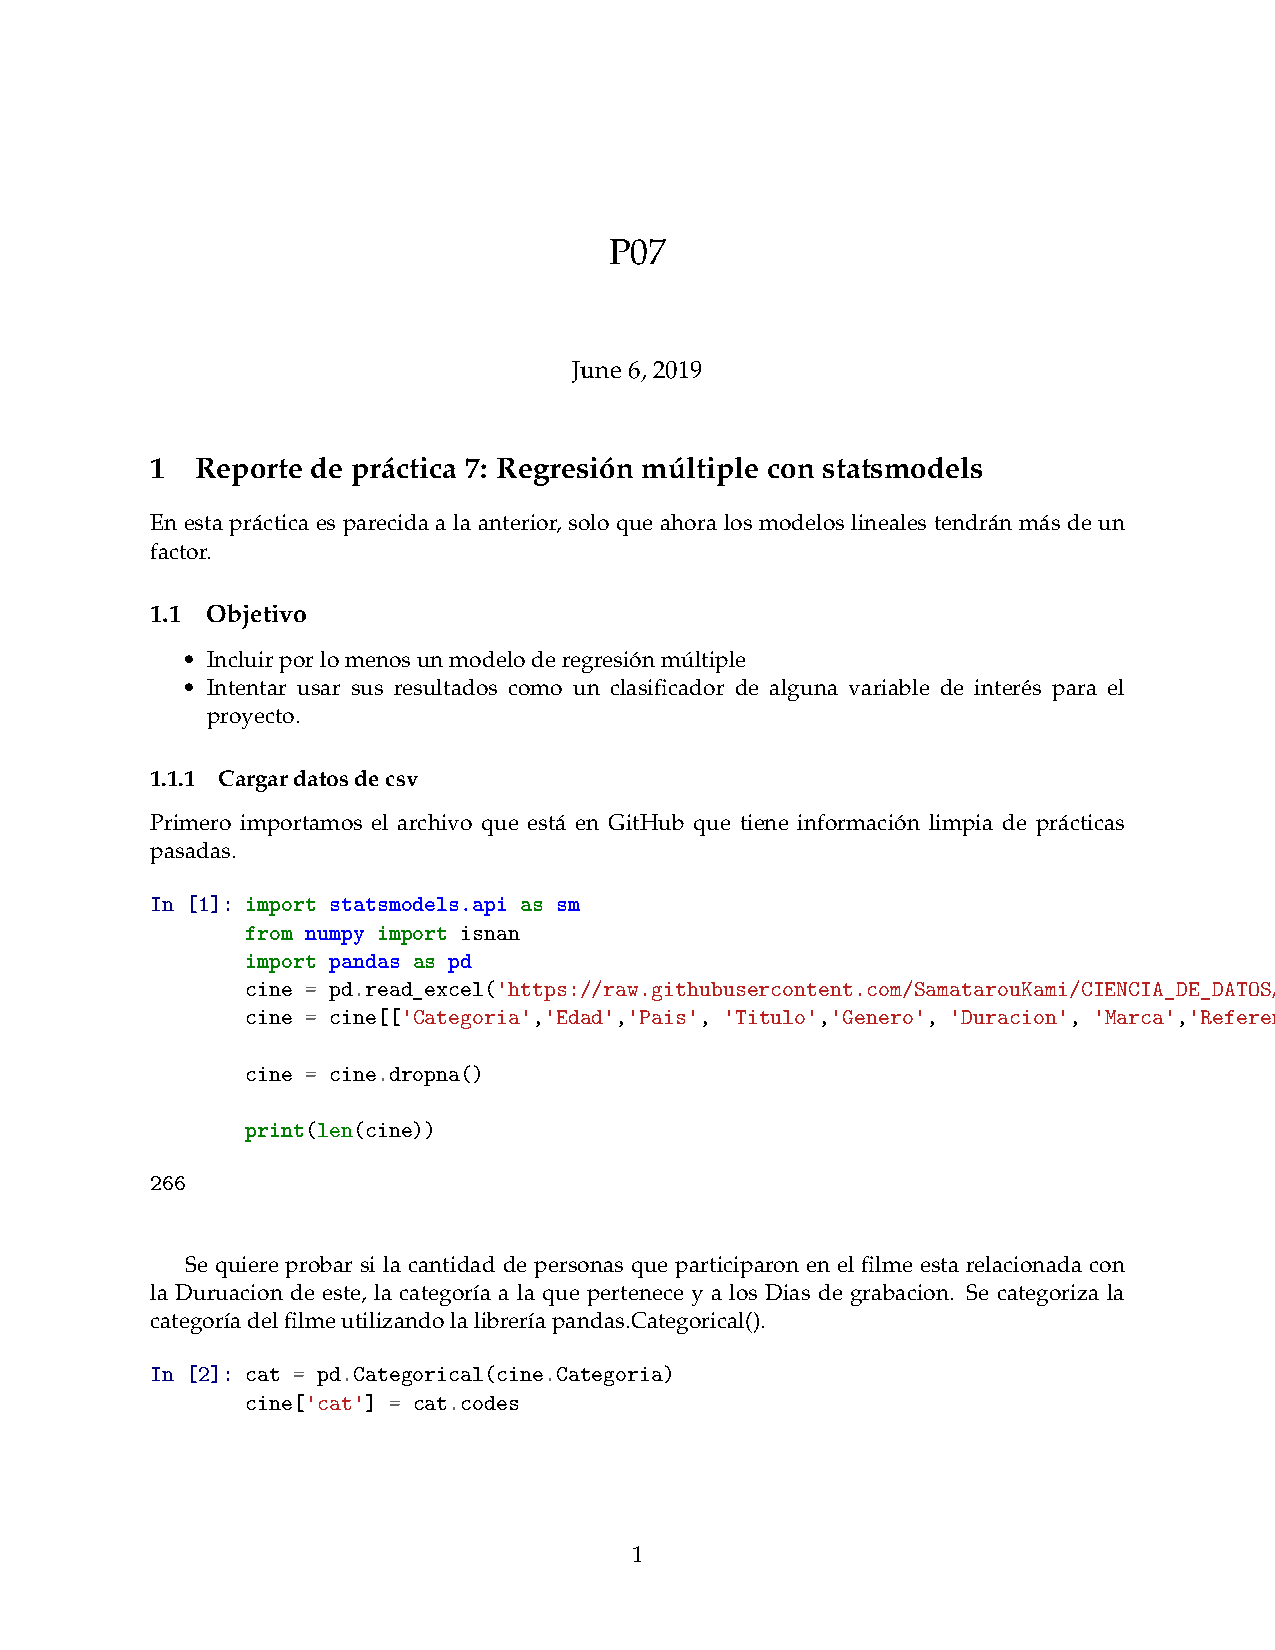
\includepdf[ pages=-, frame, scale=.85]{P07}

\chapter*{Práctica 8: Análisis de varianza y de componentes principales}
\section*{Complicaciones}

\includepdf[ pages=-, frame, scale=.85]{NP}
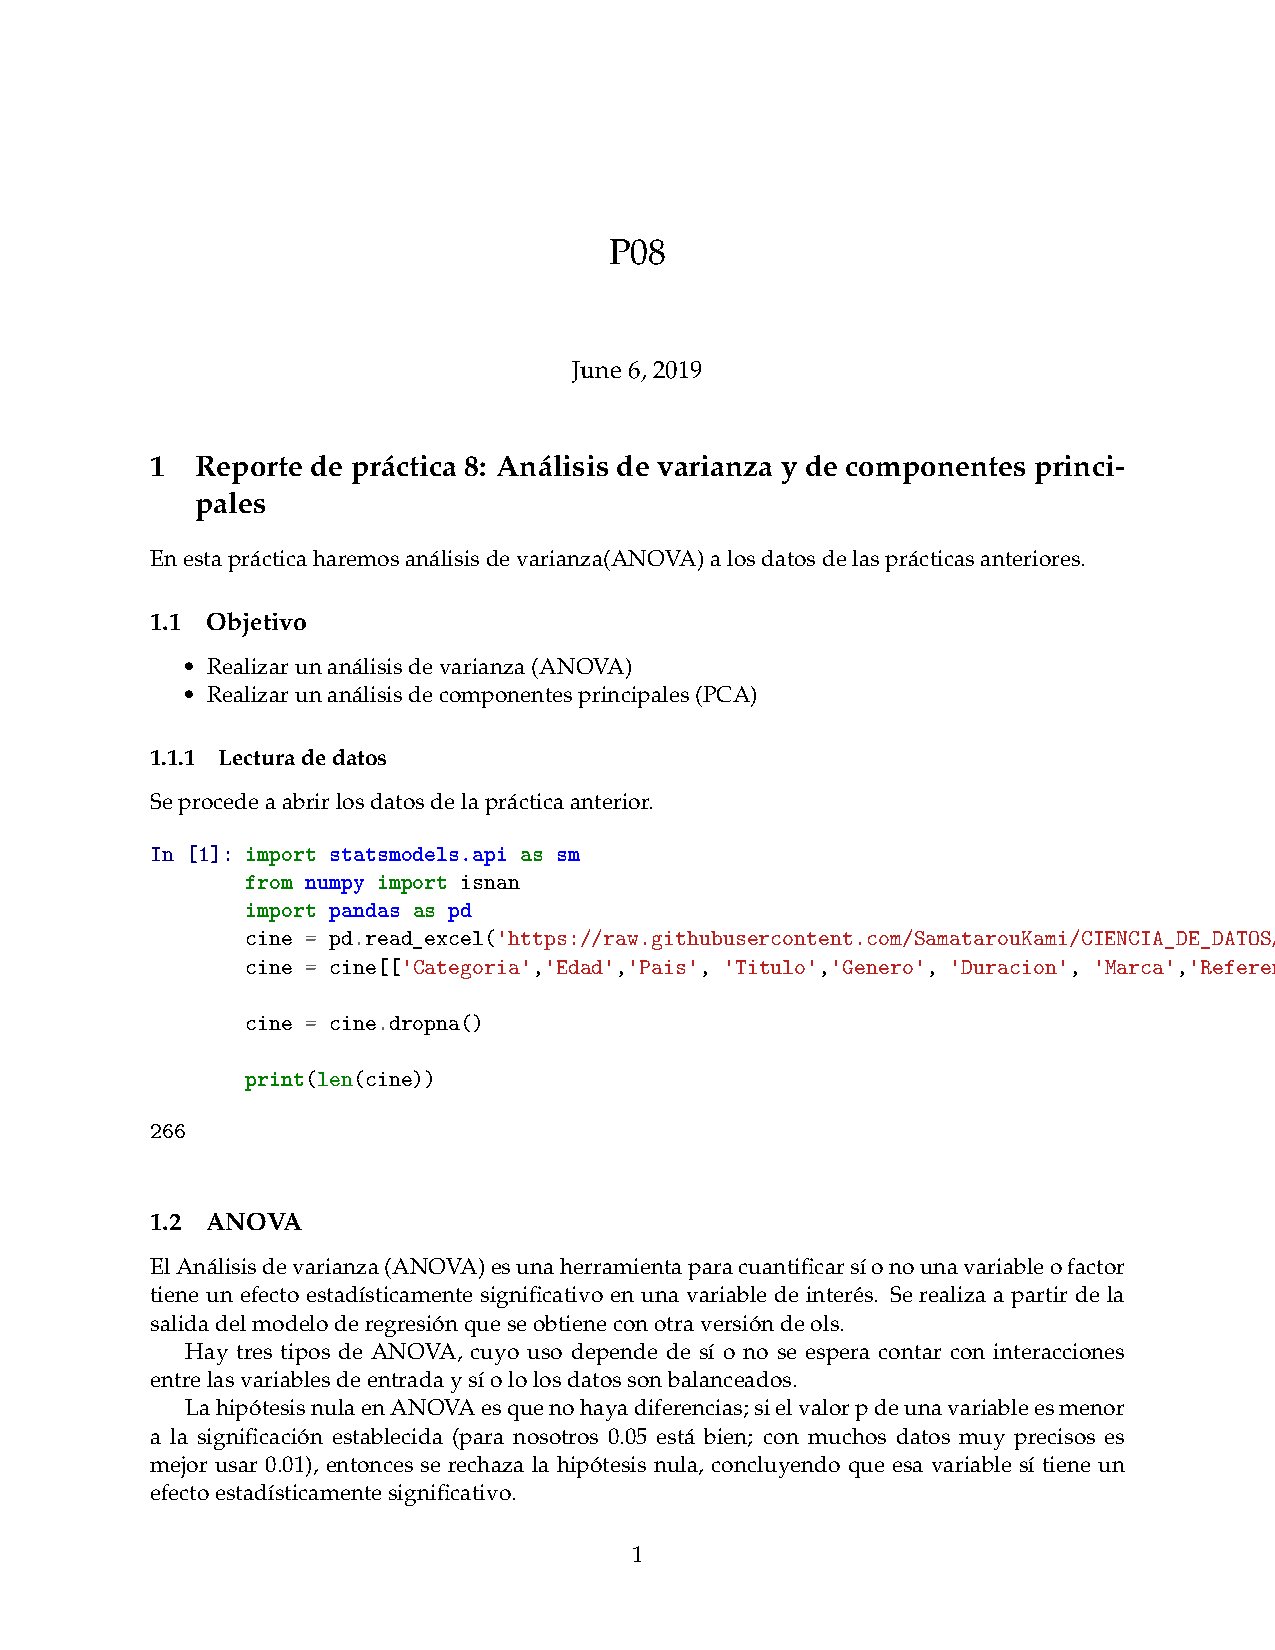
\includepdf[ pages=-, frame, scale=.85]{P08}

\chapter*{Práctica 9: Pronósticos}
\section*{Complicaciones}
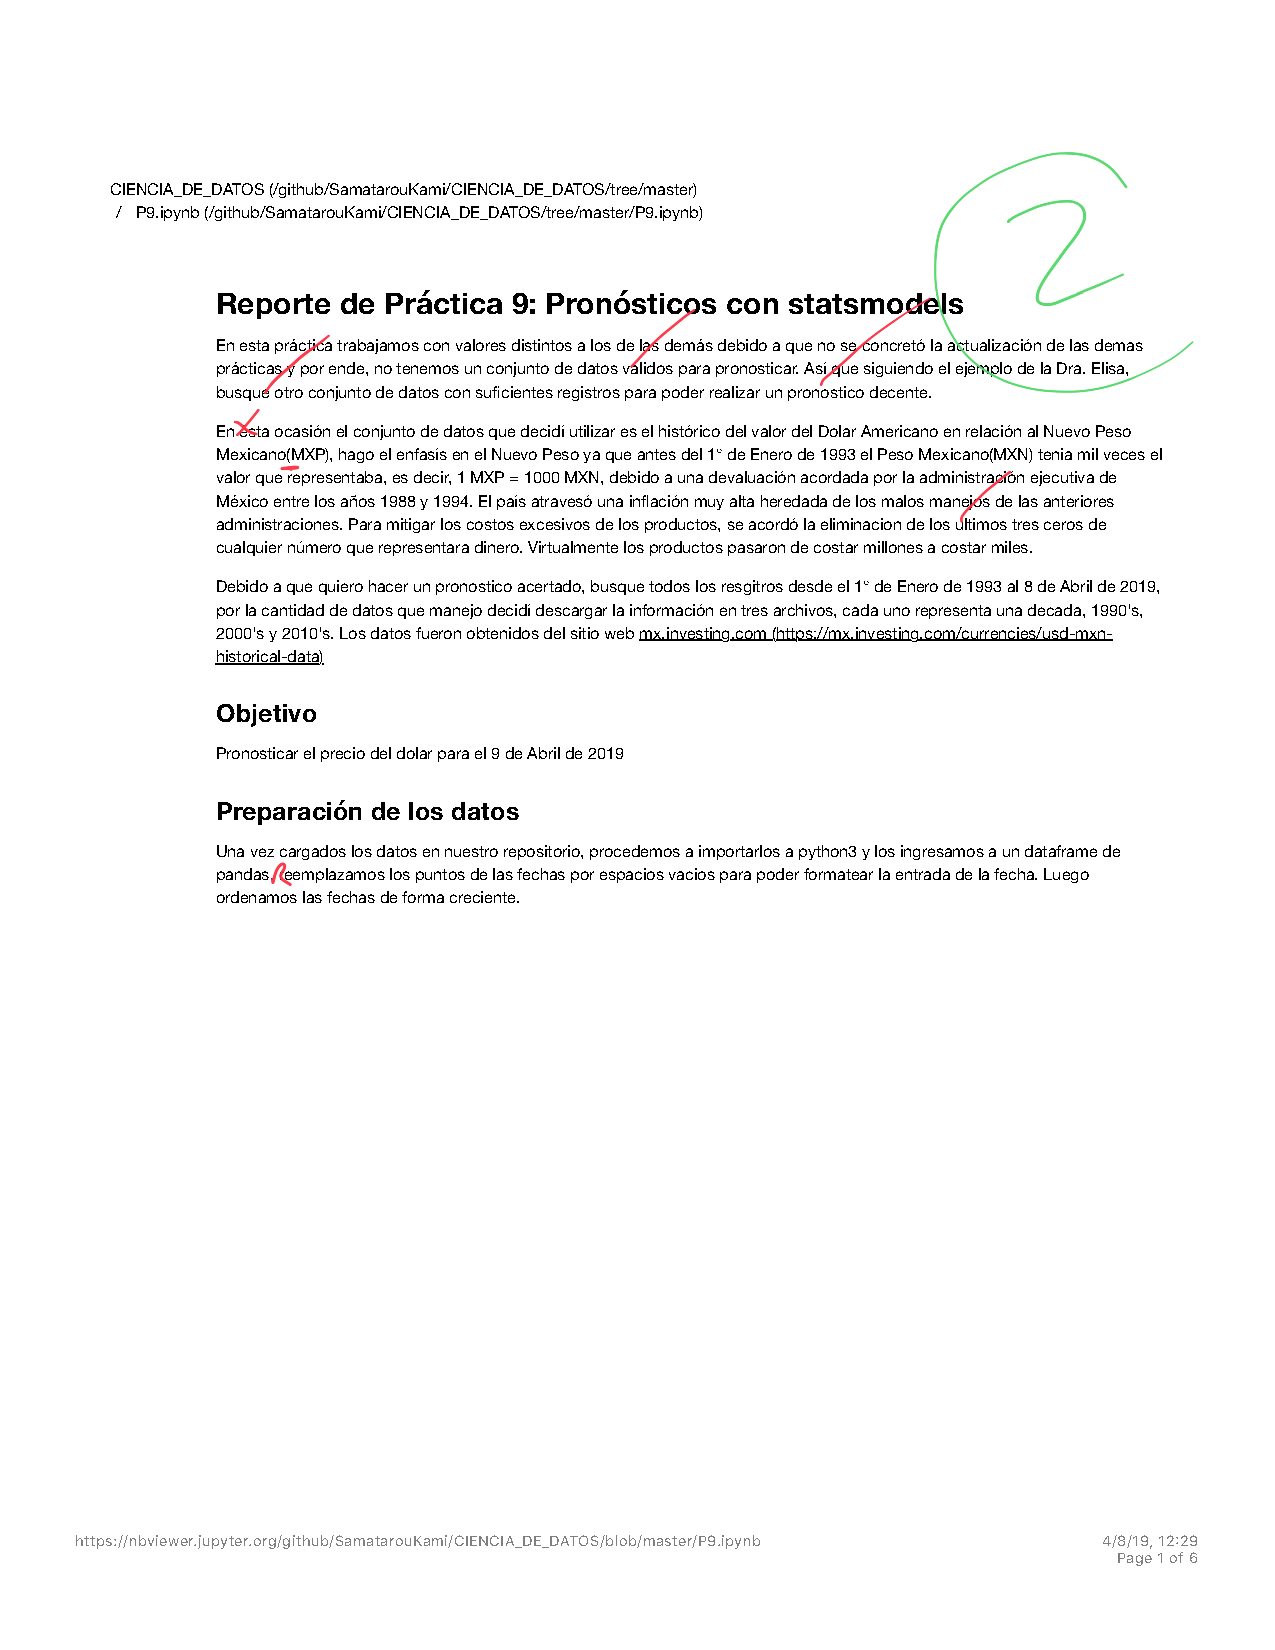
\includepdf[ pages=-, frame, scale=.85]{LA9}
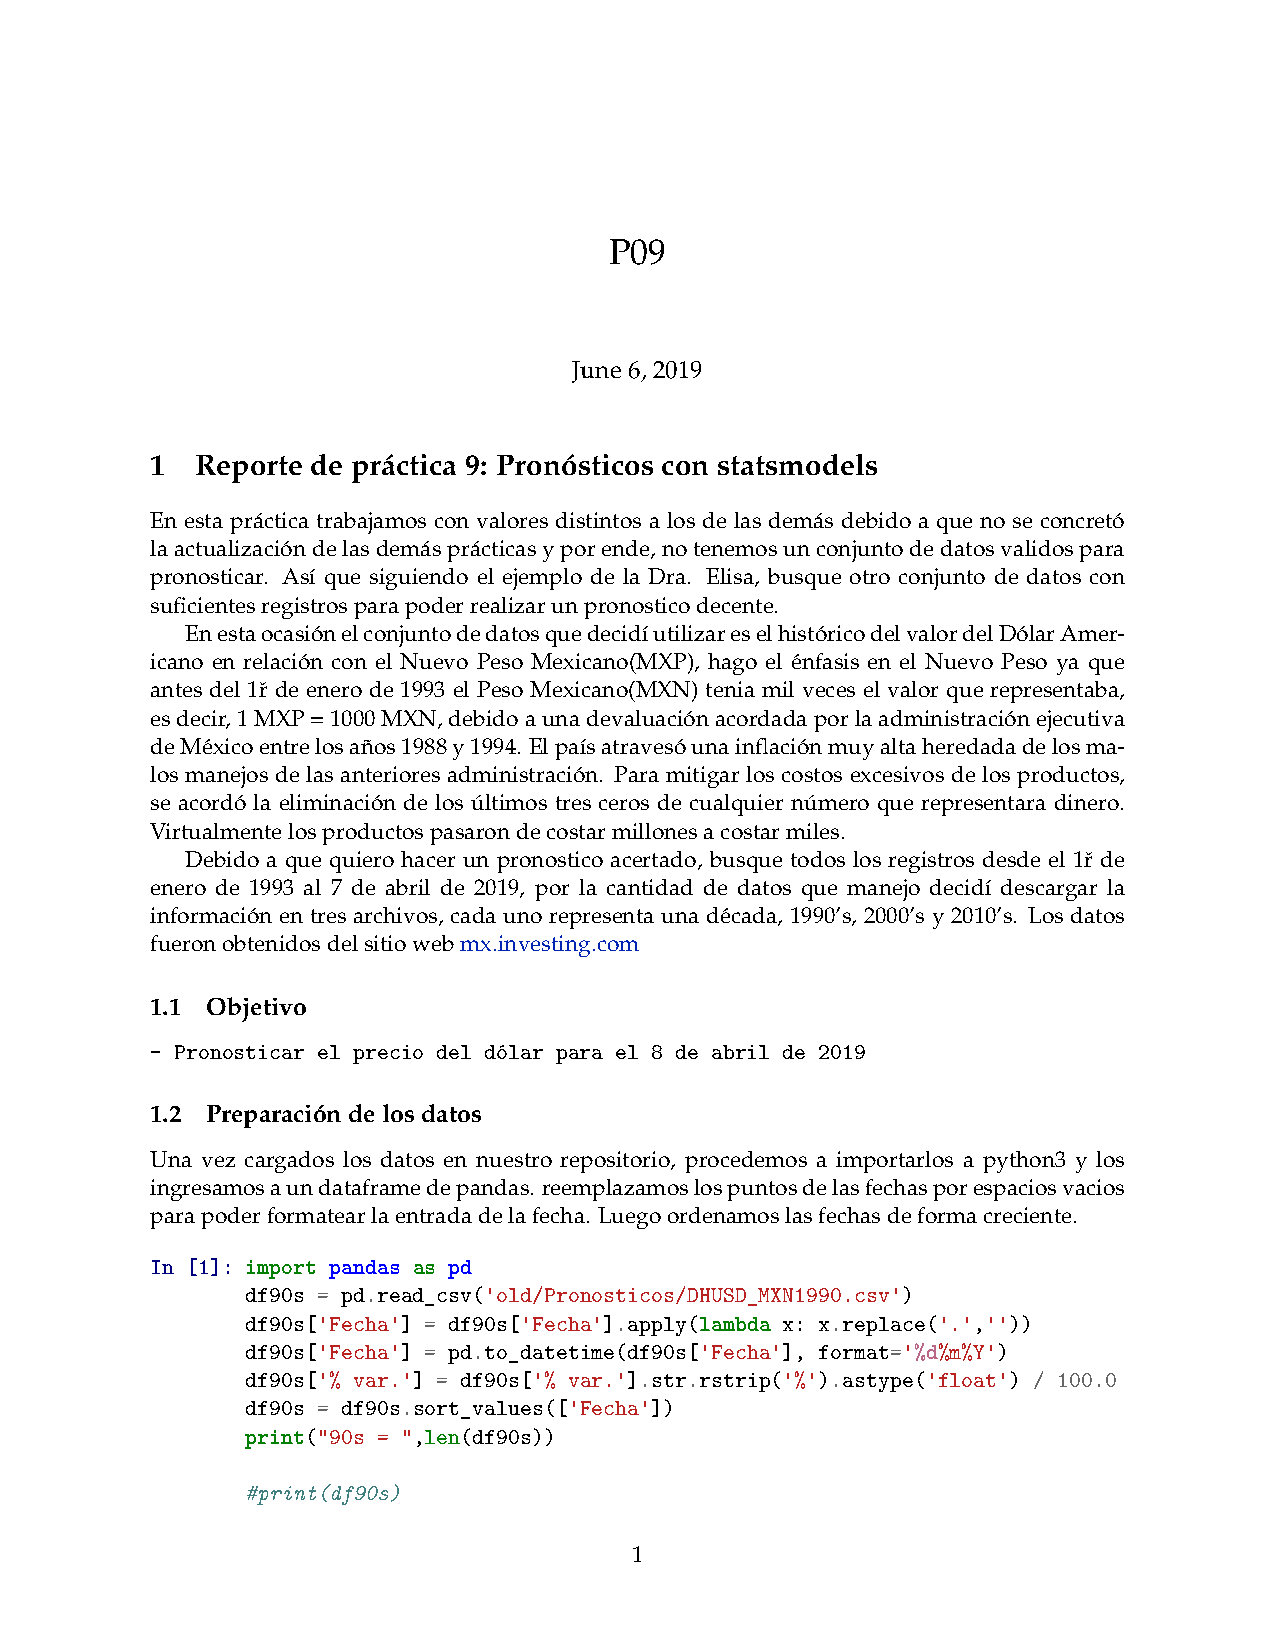
\includepdf[ pages=-, frame, scale=.85]{P09}

\chapter*{Práctica 10: Clasificación de datos}
\section*{Complicaciones}
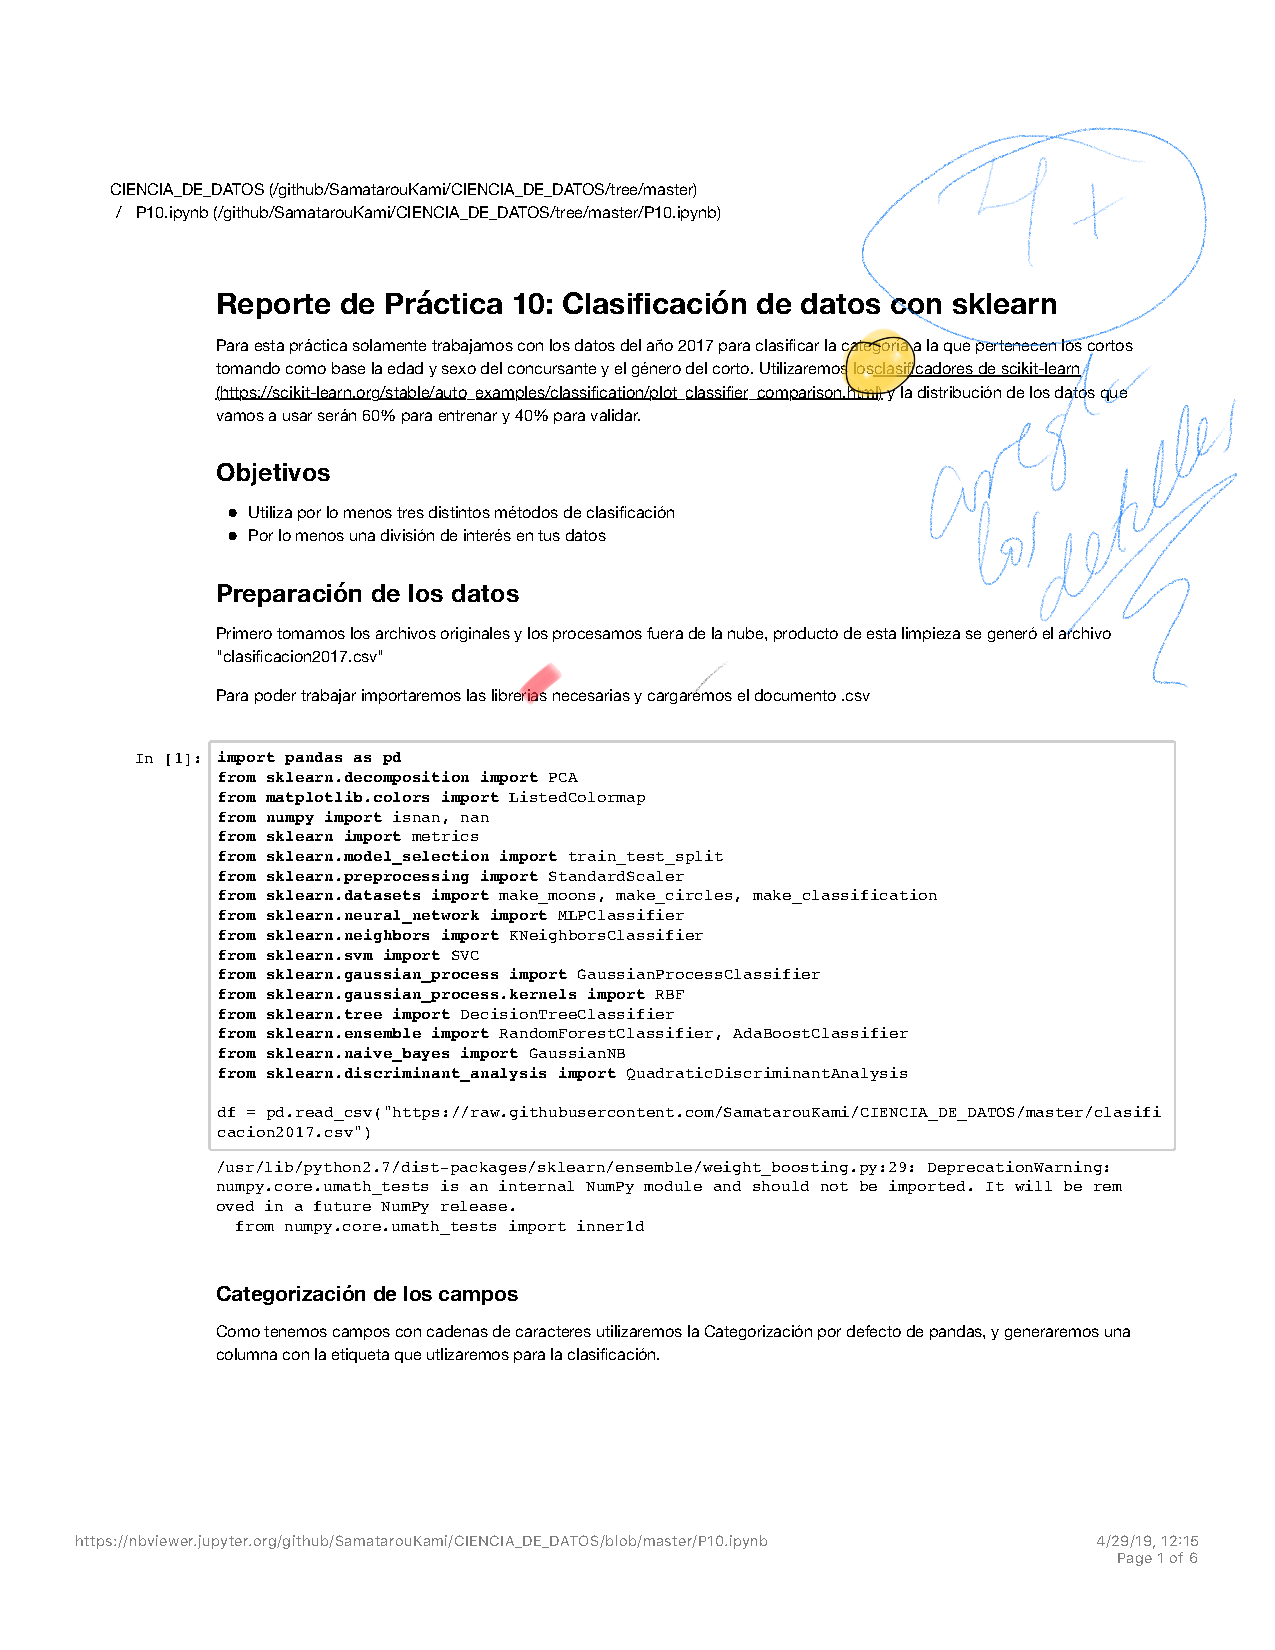
\includepdf[ pages=-, frame, scale=.85]{LA10}
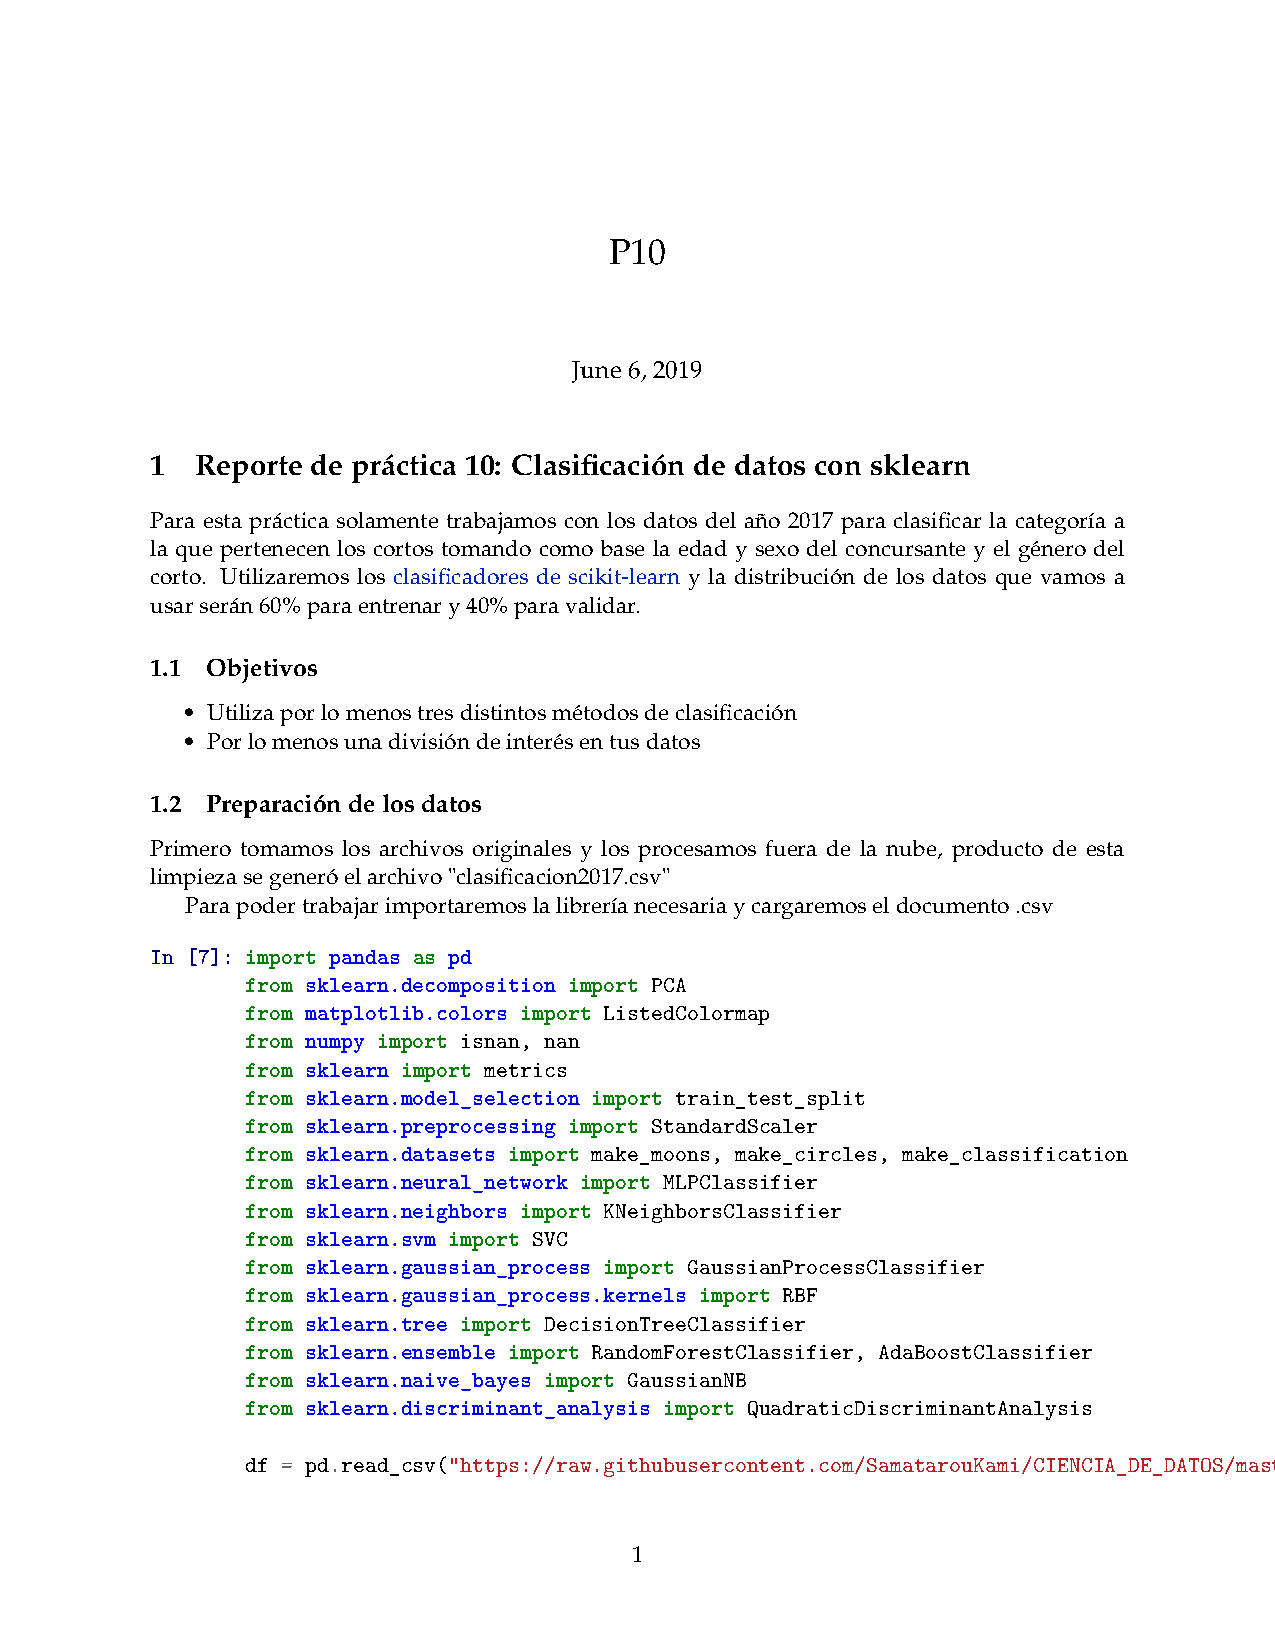
\includepdf[ pages=-, frame, scale=.85]{P10}

\chapter*{Práctica 11: Agrupamiento de datos}
\section*{Complicaciones}
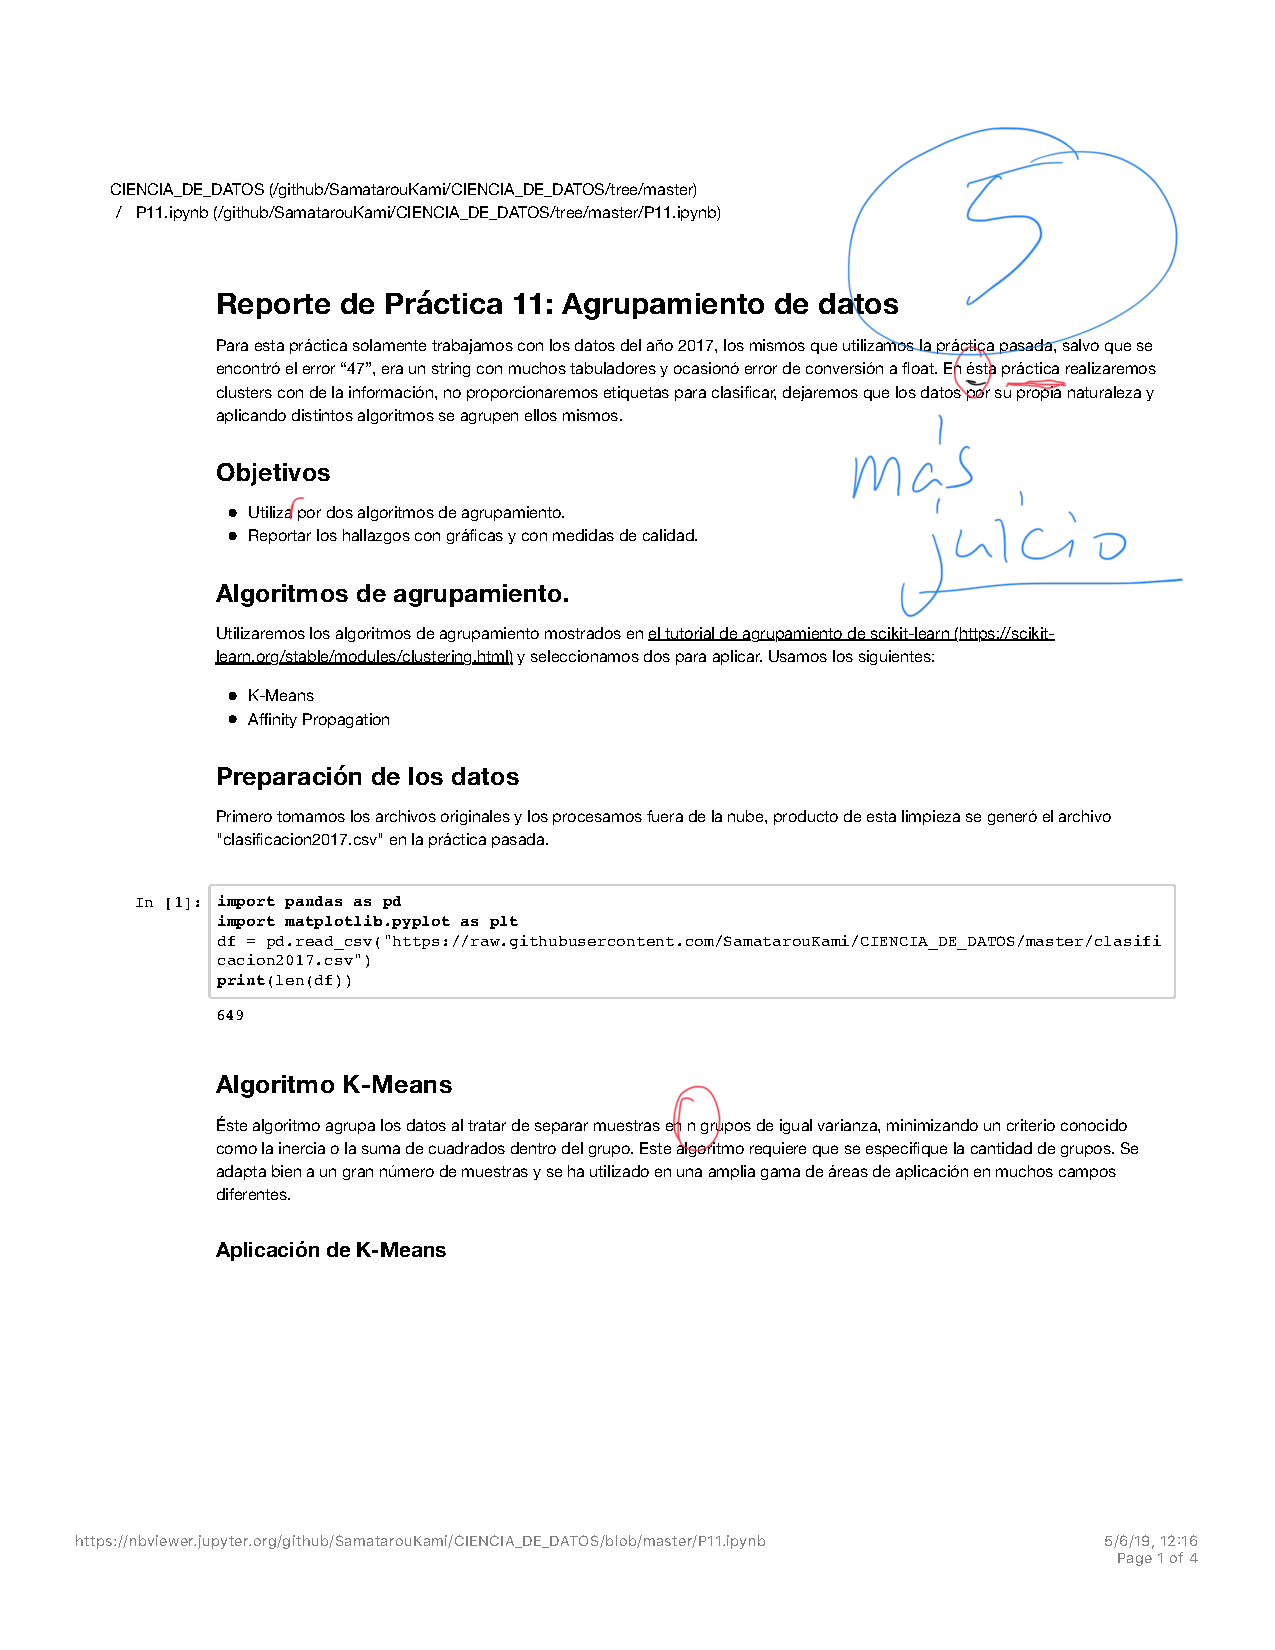
\includepdf[ pages=-, frame, scale=.85]{LA11}
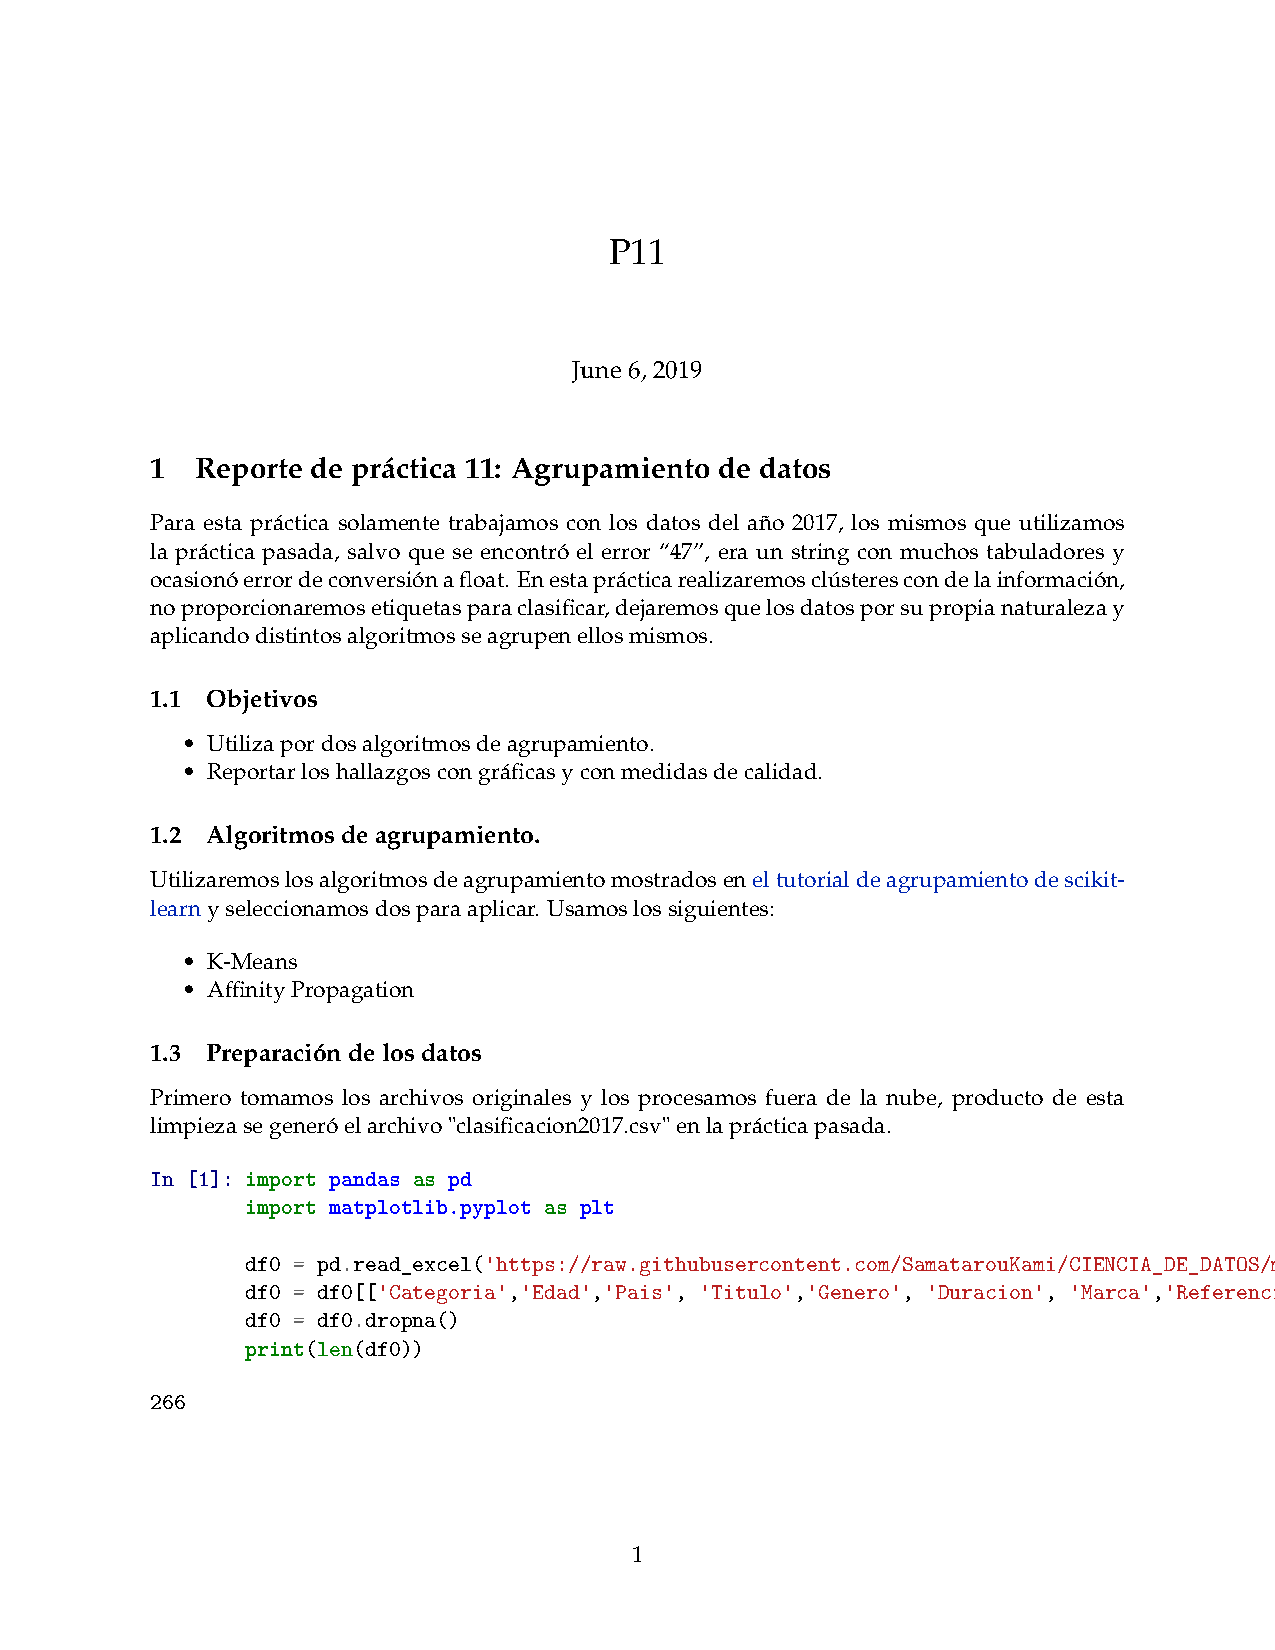
\includepdf[ pages=-, frame, scale=.85]{P11}

\chapter*{Práctica 12: Análisis de texto}
\section*{Complicaciones}

\includepdf[ pages=-, frame, scale=.85]{NP}
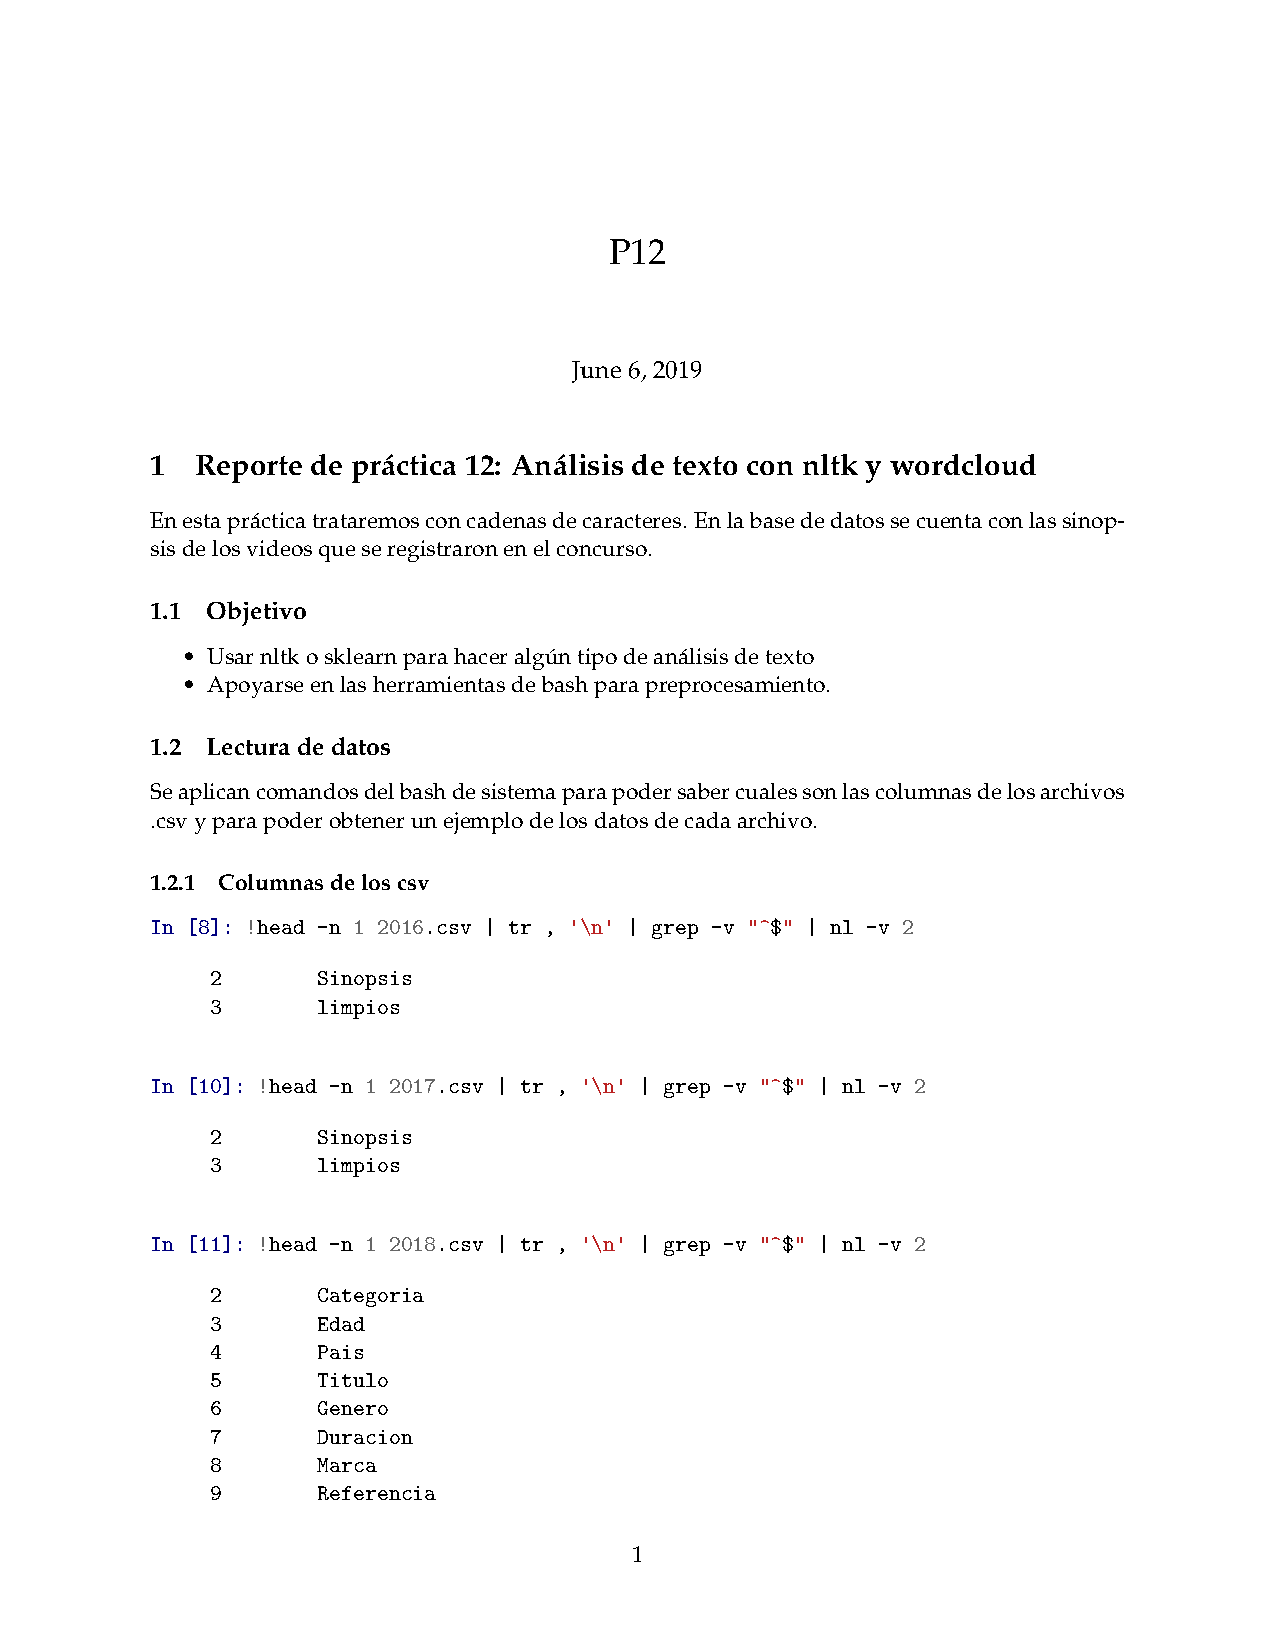
\includepdf[ pages=-, frame, scale=.85]{P12}

\chapter*{Práctica 13: Análisis de imágenes}
\section*{Complicaciones}
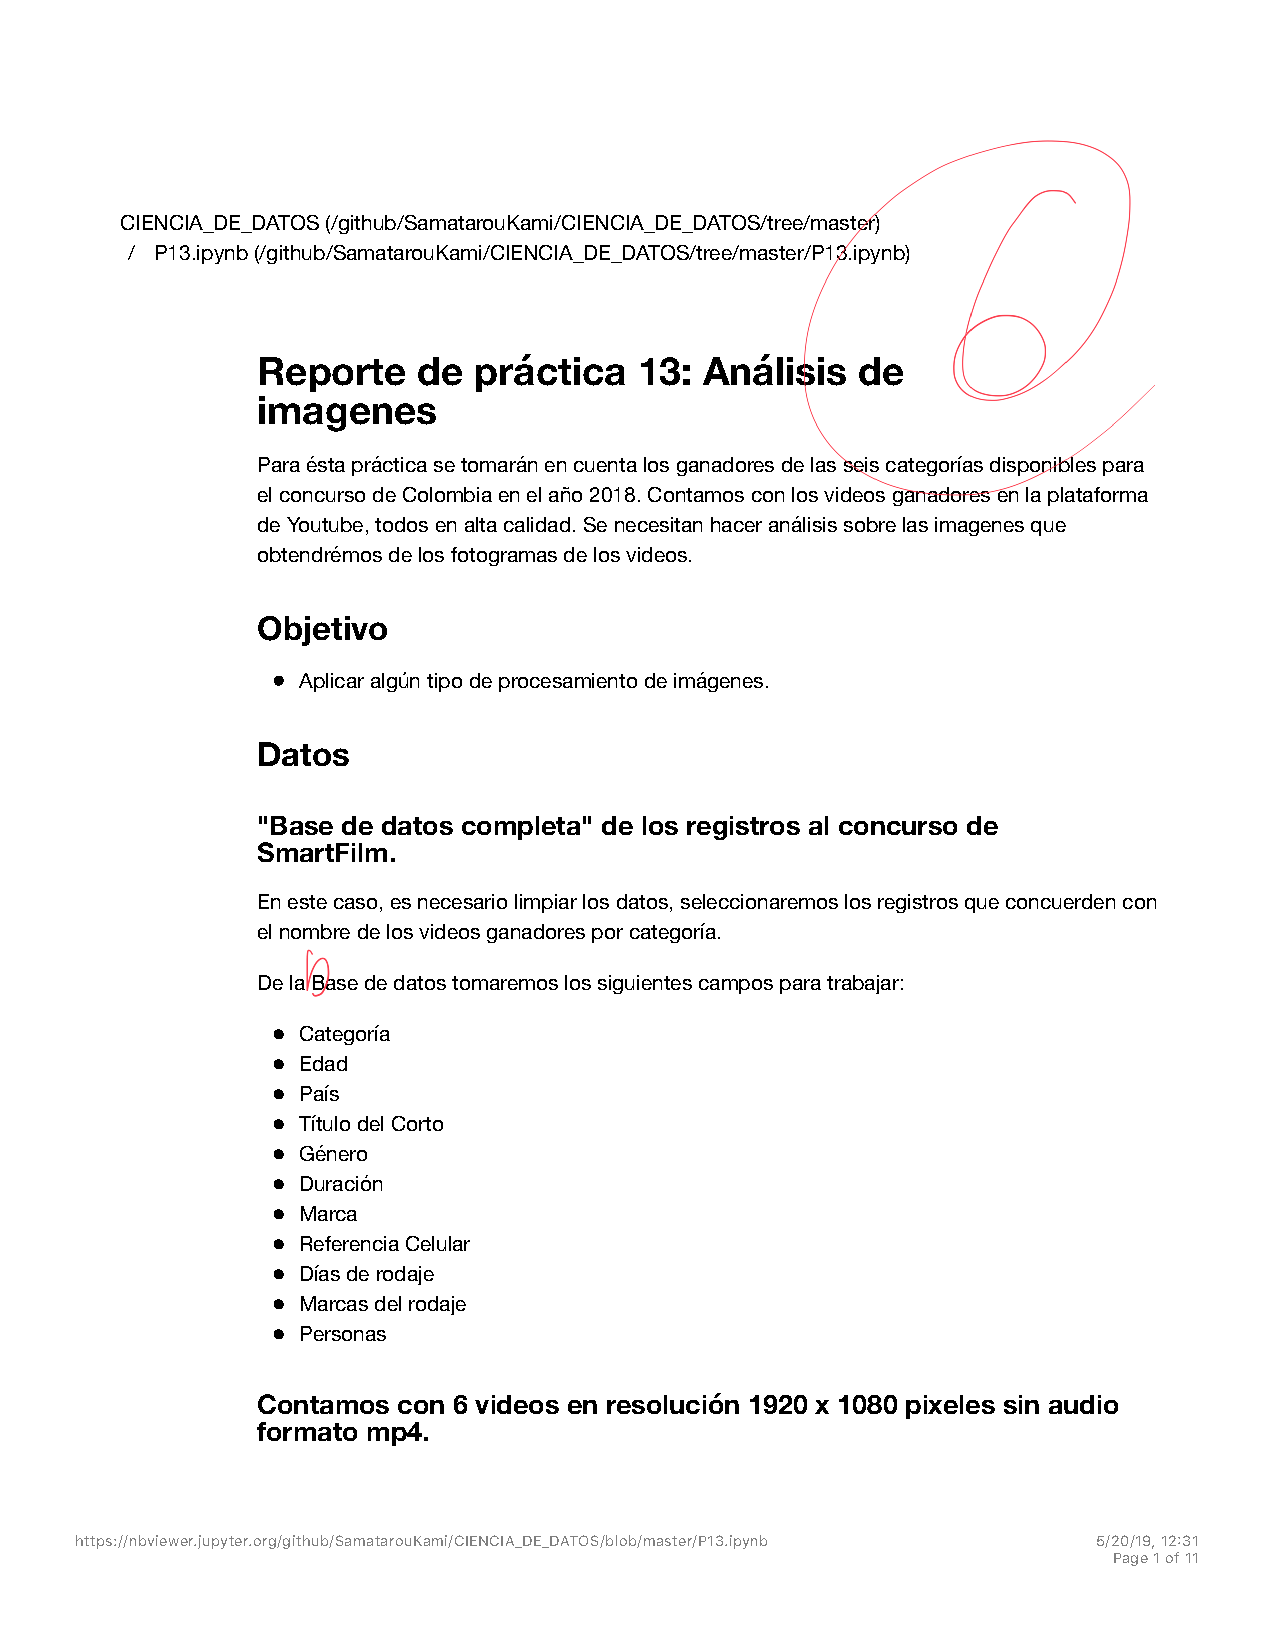
\includepdf[ pages=-, frame, scale=.85]{LA13}
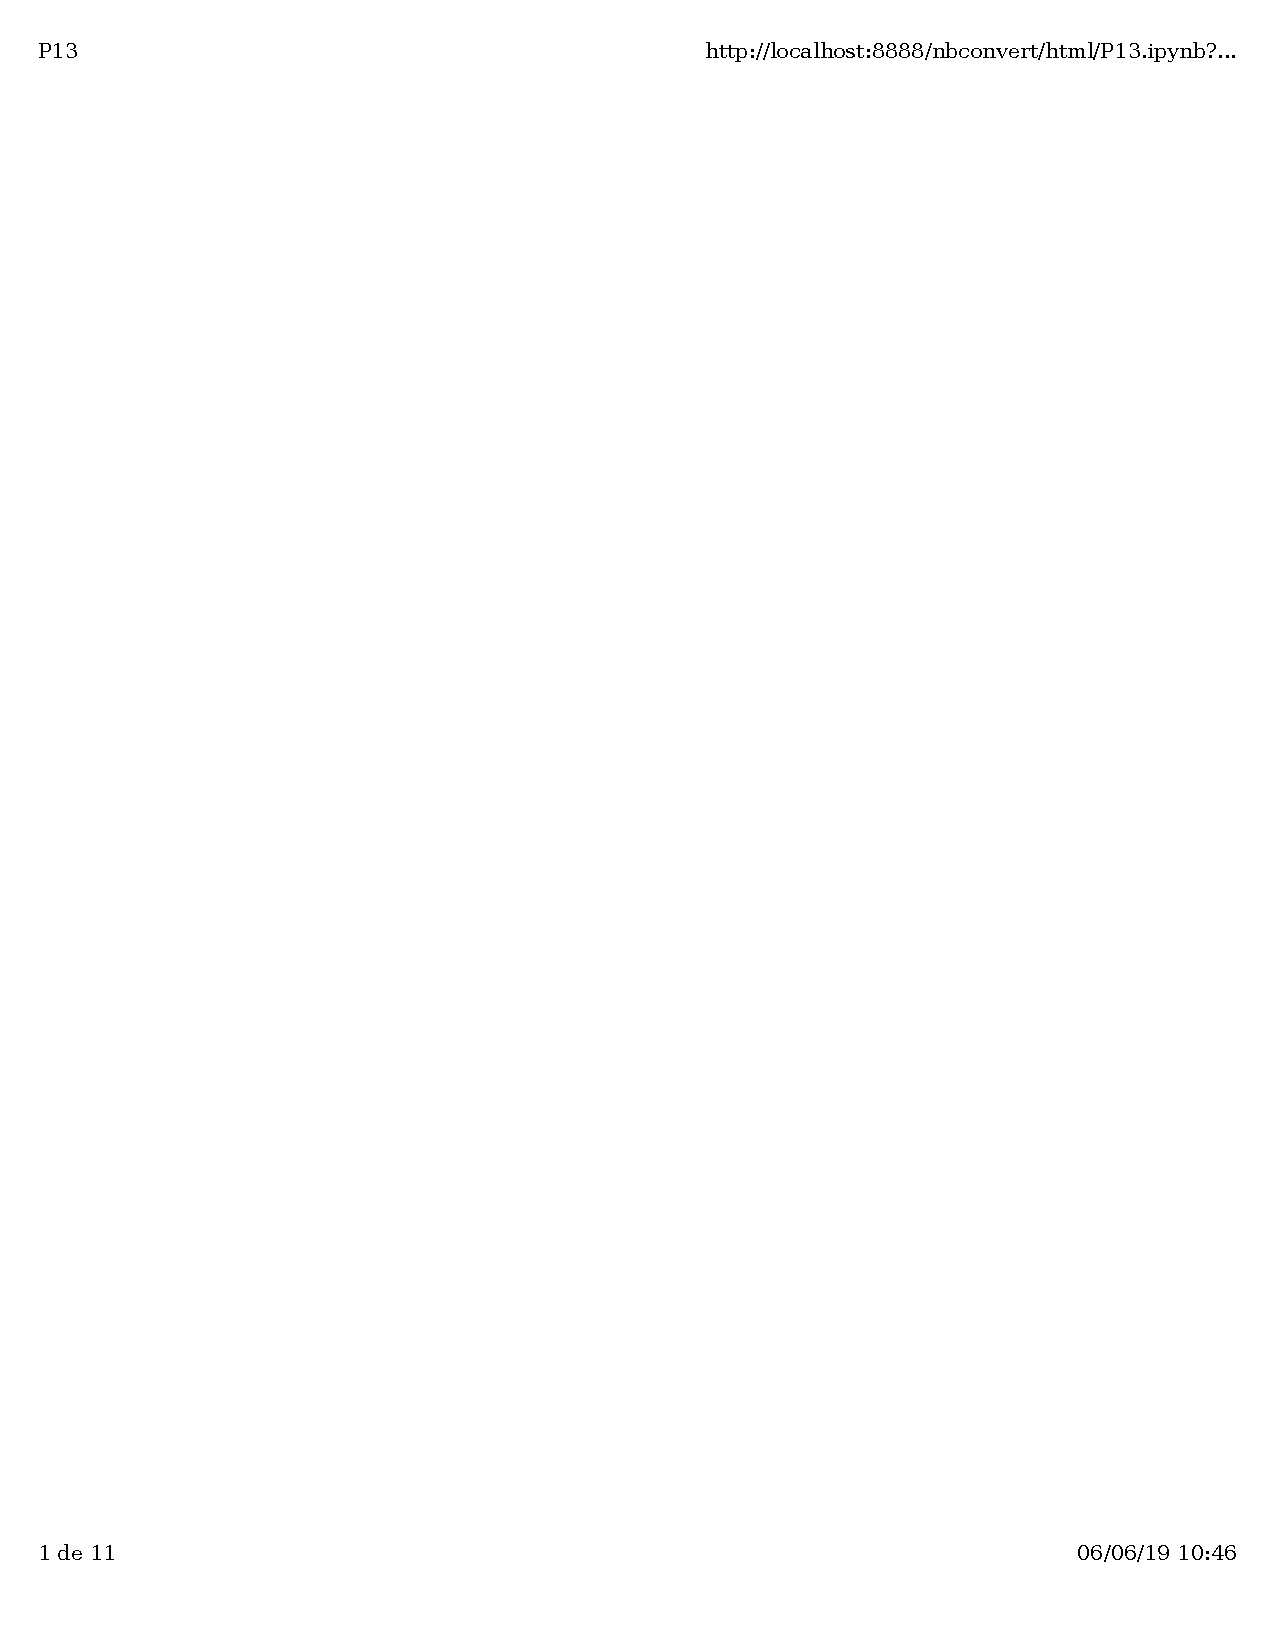
\includepdf[ pages=-, frame, scale=.85]{P13}

\chapter*{Preparación de artículo}
\section*{Complicaciones}
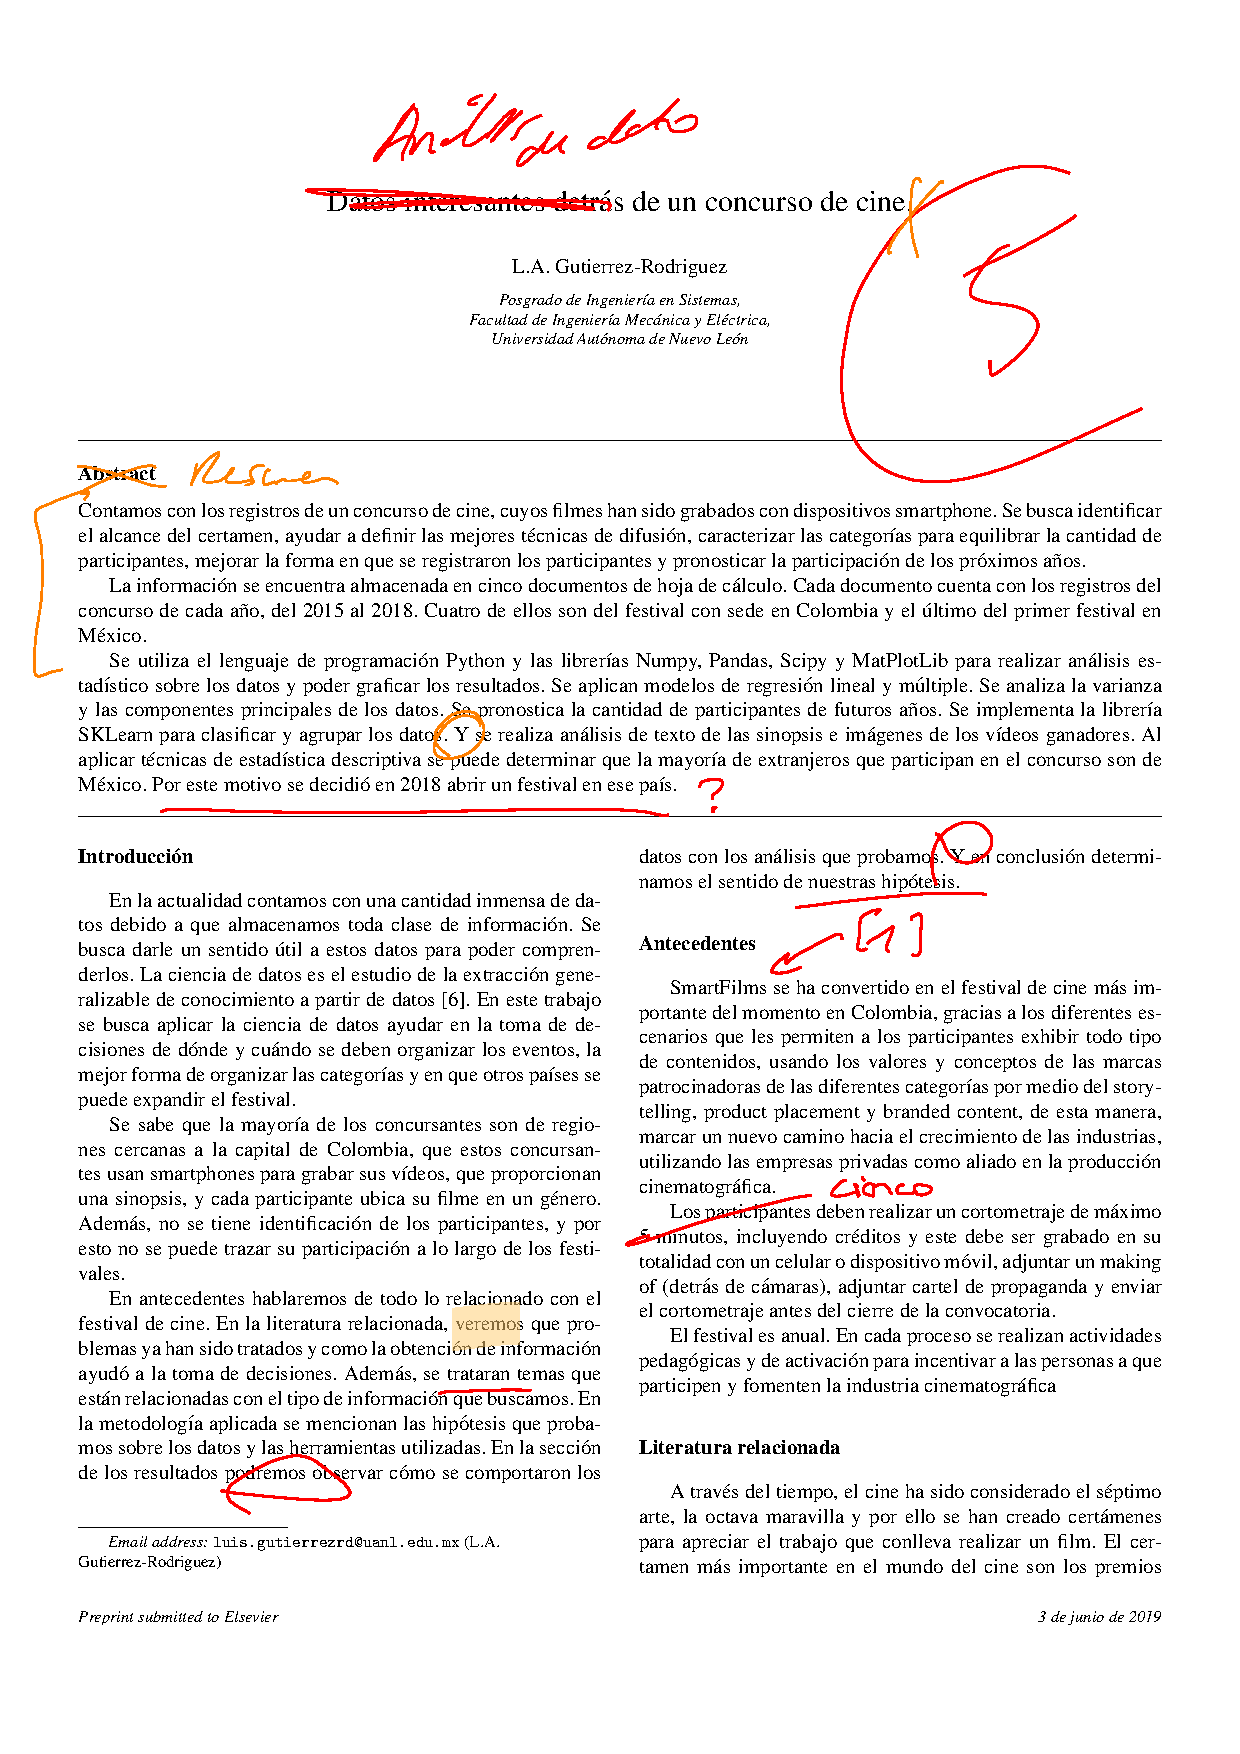
\includepdf[ pages=-, frame, scale=.85]{LAA}
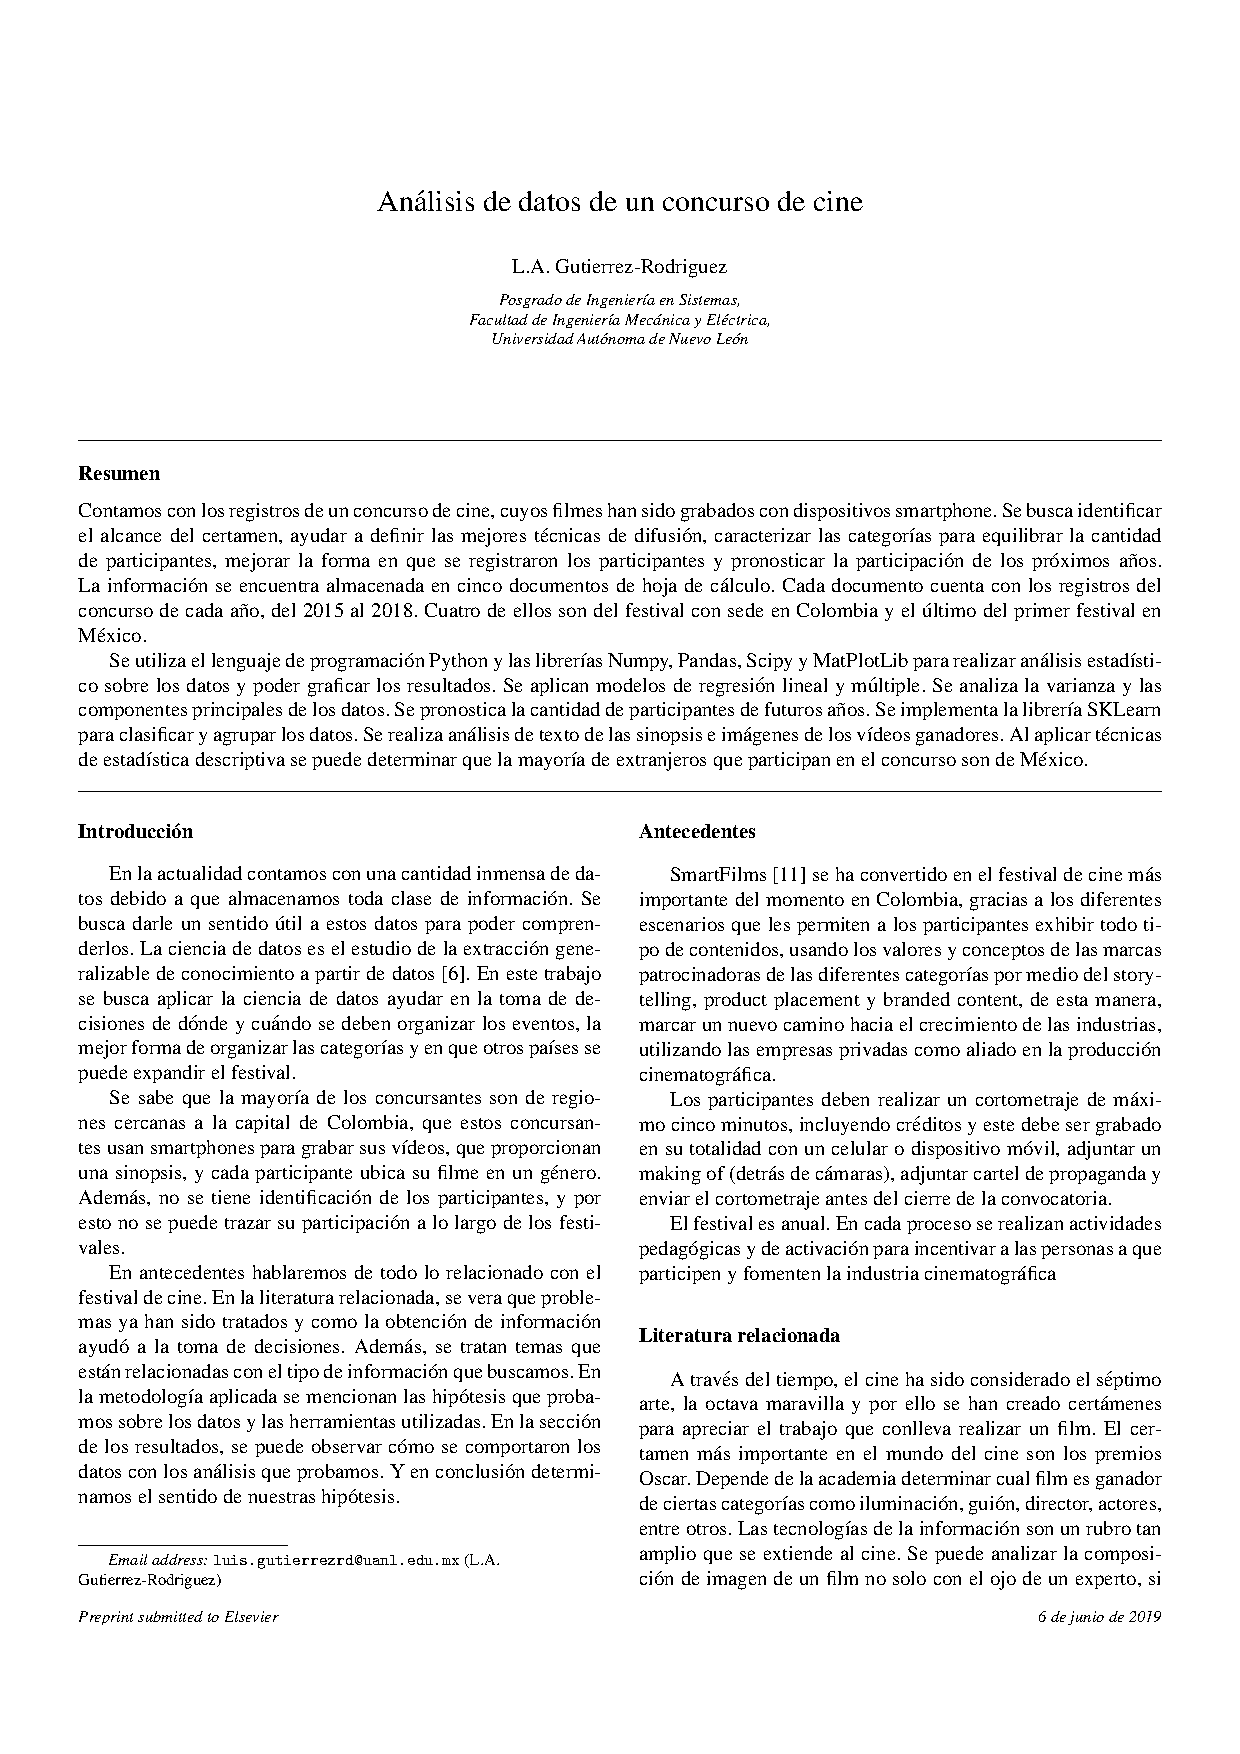
\includepdf[ pages=-, frame, scale=.85]{P14}



\end{document}